% -*- mode:flyspell; mode:latex -*-
% \documentclass[a4paper,twoside,11pt]{book}
\documentclass[12pt]{article}

\addtolength{\oddsidemargin} {-0.885in}
\addtolength{\textwidth}{1.75in}
\addtolength{\evensidemargin}{-0.8in}

\usepackage[latin1]{inputenc}
\usepackage[T1]{fontenc}
\usepackage[english]{babel}
\usepackage{float}
\usepackage{graphicx}
\usepackage{ulem}


\usepackage{tikz}
\usepackage{[caption}
\usetikzlibrary{arrows}
\usetikzlibrary{decorations.markings}
\usetikzlibrary{decorations.pathmorphing}
% \usepackage[absolute,overlay]{textpos}
% \usepackage{onimage}

\usepackage{times}

% \usepackage{subfigure}
% \usepackage{scalefnt}
% 
% \renewcommand\thesubfigure{\arabic{subfigure}}

\usepackage{amsmath}
\usepackage{hyperref}
\usepackage{hhline}
\usepackage{subfig}
\usepackage{color}
\usepackage[all]{hypcap}

% \usepackage[normalem]{ulem}  % for striking out
% \usepackage{fancyhdr}
% \pagestyle{fancy}
% \fancyhead[C]{}
% \fancyhead[L] {\it{Mu2e-doc-29670-v1.0} }
%%%%%%%%%%%%%%%%%%%%%%%%%%%%%%%%%%%%%%%%%%%%%%%%%%%%%%%%%%%%%%%%%%%%%%%%%%%%%%
% use natbib - biblatex not available on Mu2e interactive nodes
%%%%%%%%%%%%%%%%%%%%%%%%%%%%%%%%%%%%%%%%%%%%%%%%%%%%%%%%%%%%%%%%%%%%%%%%%%%%%%
\usepackage[square,sort,comma,numbers]{natbib}

% location of the .bib files: env var BIBINPUTS (~/library/bibliography)

% \usepackage[backend=biber, style=numeric-comp, sorting=ynt] {biblatex}
% \addbibresource{clfv.bib}

% \addbibresource{stntuple.bib}
% \addbibresource{mu2e_web.bib}
% \addbibresource{radiative_pion_capture.bib}

\graphicspath{{figures/}}
%%%%%%%%%%%%%%%%%%%%%%%%%%%%%%%%%%%%%%%%%%%%%%%%%%%%%%%%%%%%%%%%%%%%%%%%%%%%%%
% for portability, make sure all commands are included locally
%%%%%%%%%%%%%%%%%%%%%%%%%%%%%%%%%%%%%%%%%%%%%%%%%%%%%%%%%%%%%%%%%%%%%%%%%%%%%%
%\include{commands}
\newcommand {\kmax}            {\mbox{$k_{\rm max}$}}
\newcommand {\mumemconv}[1][A] {\mbox{$\mu^- \textrm{#1} \rightarrow e^- \textrm{#1}$}}

% Define a relay to have 2 default arguments instead of limit of 1
\newcommand {\mumepconv}[1][A] {%
  \def\ArgI{{#1}}%store the first argument
  \mumepconvRelay
}
\newcommand \mumepconvRelay[1][A]  {\mbox{$\mu^- \textrm{\ArgI} \rightarrow e^+ \textrm{#1}$}}
\newcommand {\MuToEm}     {\mbox{$\mu^- \ra e^-$}}
\newcommand {\MuToEp}     {\mbox{$\mu^- \ra e^+$}}
\newcommand {\MuPToEp}    {\mbox{$\mu^+ \ra e^+$}}

\newcommand {\ra}        {\rightarrow}
\newcommand {\red}       {\color{red} }
\newcommand {\blue}      {\color{blue}}
\newcommand {\tandip}    {\mbox{$\tan \lambda$}}

\newcommand {\Pb}[1]     {\mbox{$\rm ^{#1}Pb$}}                 % isotopes of lead
\newcommand {\Au}[1]     {\mbox{$\rm ^{#1}Au$}}                 % isotopes of gold
\newcommand {\Ir}[1]     {\mbox{$\rm ^{#1}Ir$}}                 % isotopes of iridium

\newcommand {\strike}[1] {{\blue \sout{#1}}}
%%%%%%%%%%%%%%%%%%%%%%%%%%%%%%%%%%%%%%%%%%%%%%%%%%%%%%%%%%%%%%%%%%%%%%%%%%%%%%
\begin{document}

\begin{titlepage}
  \begin{flushright}
    \bf {MU2E/PHYSICS/36375} \\
    version 1.02
    \today
 \end{flushright}

  \vspace{1cm}
  
  \begin{center}
    {\Large \bf Mu2e 2020 sensitivity update. \\
      \vspace {0,2in} 
      2. Reconstruction} 
    
    \vspace{1cm}
    
    S. Di Falco (INFN Pisa), S. Huang (Purdue Univ.,
    M. MacKenzie (Northwestern Univ.),
    P. Murat(FNAL)
    
    % \footnote{\texttt{Fermilab; e-mail: murat@fnal.gov}}
    \vspace{0.3cm}
    
    \vspace{0.8cm}                           
  \end{center}

  \begin{abstract}
    This note documents changes made to the Mu2e reconstruction software
    used for 2020 sensitivity update (SU2020).
  \end{abstract}

\end{titlepage}
% \frontmatter
% \chapter*{Abstract}
%
% \addcontentsline{toc}{chapter}{Abstract}
%
% \mainmatter
%
{\tableofcontents}

%%%%%%%%%%%%%%%%%%%%%%%%%%%%%%%%%%%%%%%%%%%%%%%%%%%%%%%%%%%%%%%%%%%%%%%%%%%%%%%
%\chapter{Calibration}
%%%%%%%%%%%%%%%%%%%%%%%%%%%%%%%%%%%%%%%%%%%%%%%%%%%%%%%%%%%%%%%%%%%%%%%%%%%%%%%
% \input{input_data}

%%%%%%%%%%%%%%%%%%%%%%%%%%%%%%%%%%%%%%%%%%%%%%%%%%%%%%%%%%%%%%%%%%%%%%%%%%%%%%%

\newpage
\section { Introduction}
The simulation and reconstruction software used for SU2020 analyses is based on
the Mu2e Offline tag v9\_0\_5, the starting point for the {\bf su2020} branch
of the Mu2e Offline.
In this note we will summarize  the most important software changes with respect to
the base tag and describe several issues uncovered along the way, which do not
affect the sensitivity estimates but need to be fixed nevertheless. 
The latter are highlighted in red and summarized in Section \ref{sec:to_be_investigated}.

All datasets referred to in this note are described in \cite{MU2E_36372_SU2020_DATASETS}. 

% -*- mode:latex; mode:flyspell -*-
%%%%%%%%%%%%%%%%%%%%%%%%%%%%%%%%%%%%%%%%%%%%%%%%%%%%%%%%%%%%%%%%%%%%%%%%%%%%%%
\section{Correcting relative tracker-calorimeter timing offset}

In an event which has a calorimeter cluster matching to a reconstructed track, the
cluster is included into the track fit as an additional hit. The algorithm reconstructing 
straw hits in the tracker and the algorithm reconstructing the waveform timing in the calorimeter
could add different timing offsets to the reconstructed hits and clusters correspondingly.
Those offsets need to be calibrated out.

A cluster is included into the track fit with the coordinate error $\sigma_{XY} = 15$ mm
and the timing error $\sigma_T = 0.5$ ns.

The distribution of the calorimeter cluster timing residuals for conversion electrons and default Kalman fit 
configuration is shown in Figure \ref{fig:track_cluster_dt}.a. The distribution of cluster timing residuals 
is centered at about -1.17 ns and has a width of about 0.34 ns, indicating presence of the systematic effect.

To study the effect and avoid biasing the fit, the errors assigned to the cluster were increased to $10^6$ (ns or mm),
the corresponding distribution in timing residuals is shown in Figure \ref{fig:track_cluster_dt}.b. 
In this case, inclusion of the cluster into the track fit doesn't bias the result of the fit and one can conclude 
that there is a systematic timing offset between the tracker and the calorimeter, which value is about 1.6 ns.

Figure \ref{fig:track_cluster_dt}.c corresponds to the fit configuration with the cluster time corrected by 1.6 ns, 
and still large errors, and one can see that the applied correction zeroes the timing offset.

Distribution of timing residuals with the cluster time corrected by 1.6ns and default errors (0.5ns and 15mm) 
assigned to the cluster shows a systematic shift of about 0.5-0.6ns, apparently introduced by the fitting procedure.

For now, we correct the cluster timing and use the default resolutions assigned to the calorimeter cluster 
in the Kalman fit.

{\red insert here from next section:
The resolution tuning has been performed after the global track-to-calorimeter timing offsets
have been corrected. The global correction introduced was 1.86ns, while after the tuning, the offset
value is about 1.6 ns. Resulting non-accounted for systematic offset of about 0.25 ns is however
about x2 smaller than the offset introduced by the Kalman fitter. }

It is worth noting that the width of the distribution in timing residual is approximately 0.5 of the error assigned 
to the cluster, which is another indication of the cluster introducing a non-compensated systematic effect into the 
Kalman fit.

\begin{figure}[h]
  \hspace{-0.8in}
  \begin{tikzpicture}
    \node[anchor=south west,inner sep=0] at (0,0.) {
      % \node[shift={(0 cm,0.cm)},inner sep=0,rotate={90}] at (0,0) {}
      % \makebox[\textwidth][c] {
      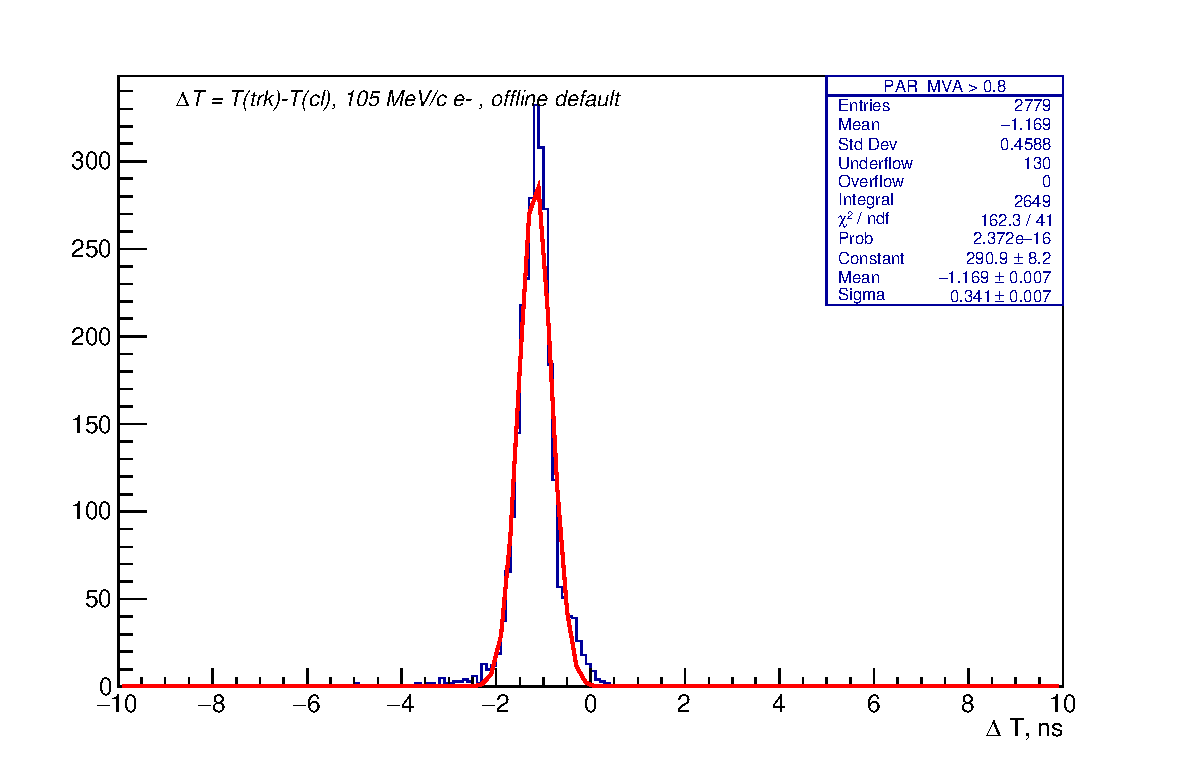
\includegraphics[width=0.64\textwidth]{figures/pdf/figure_00131_ele00s51b0_su2020_track_ana_trk_200_dt}
      % }
    };
    \node [text width=1cm, scale=0.8] at (3.,5) {(a)};
    \node[anchor=south west,inner sep=0] at (10.7,0.) {
      % \node[shift={(0 cm,0.cm)},inner sep=0,rotate={90}] at (0,0) {}
      % \makebox[\textwidth][c] {
      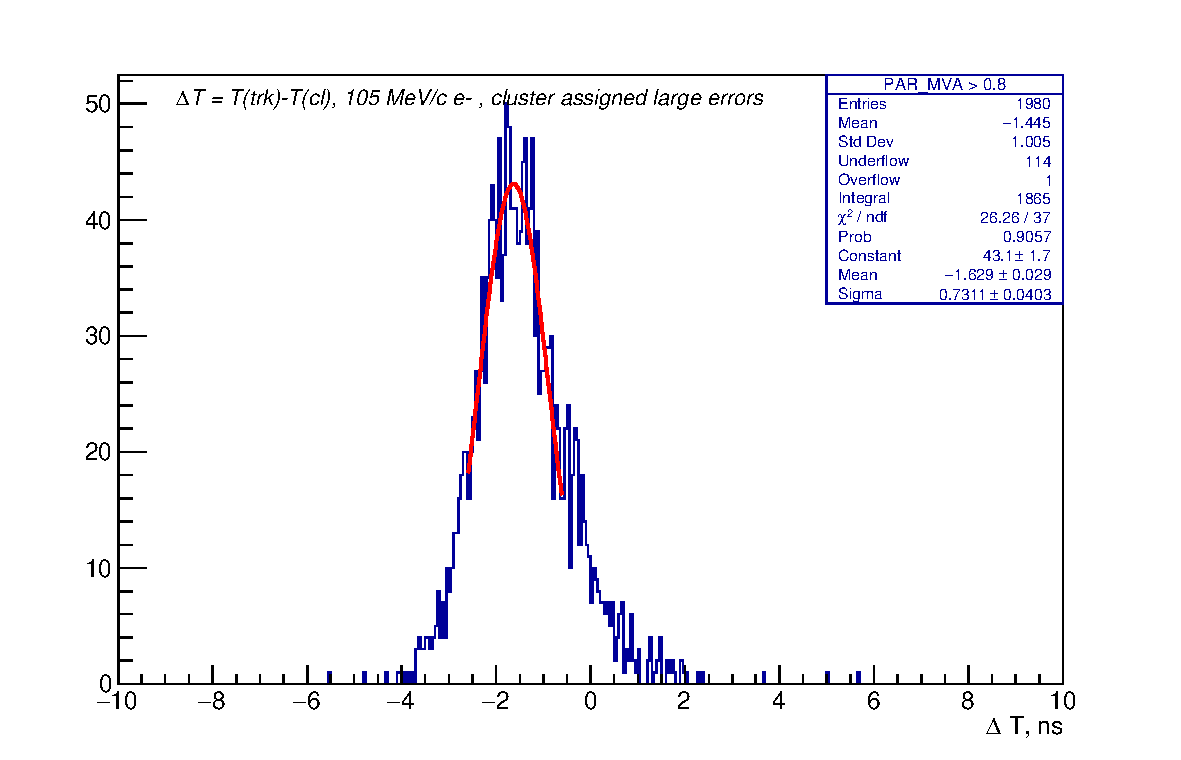
\includegraphics[width=0.64\textwidth]{figures/pdf/figure_00132_ele00s51b0_pid_emuana_trk_101_dt}
      % }
    };
    \node [text width=1cm, scale=0.8] at (13.7,5) {(b)};
    \node[anchor=south west,inner sep=0] at (0,-7.0) {
      % \node[shift={(0 cm,0.cm)},inner sep=0,rotate={90}] at (0,0) {}
      % \makebox[\textwidth][c] {
      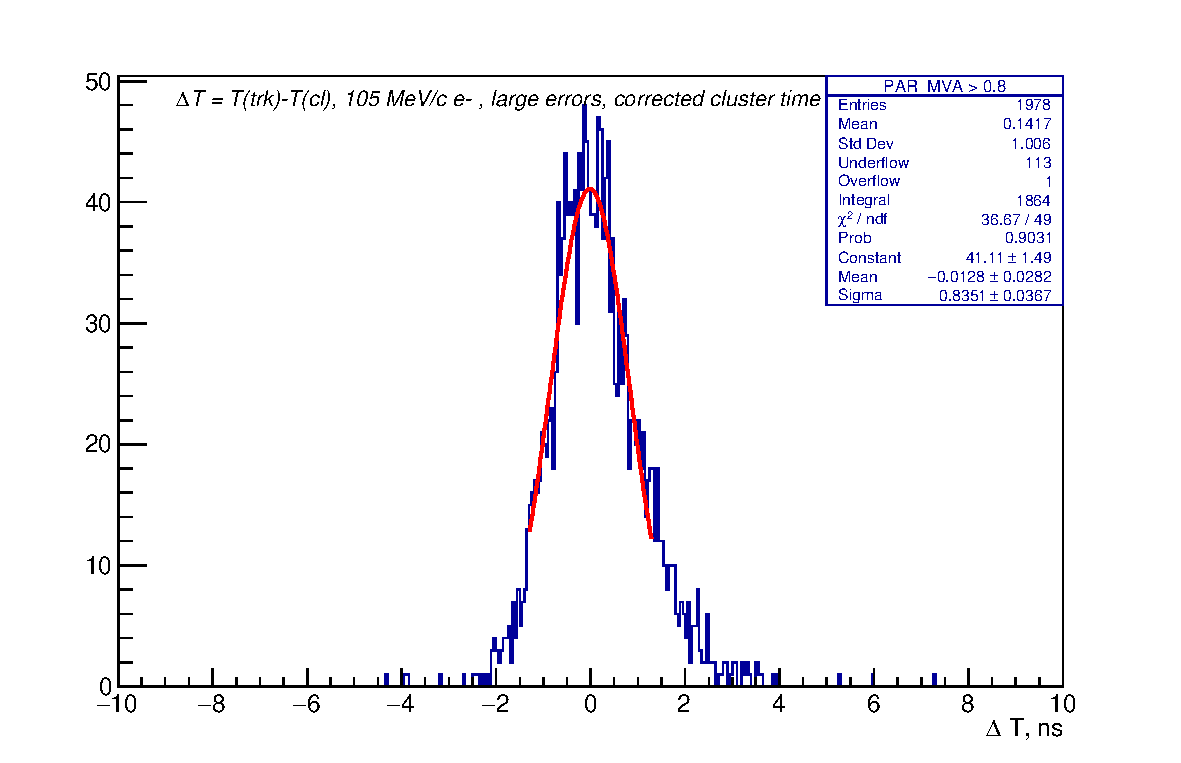
\includegraphics[width=0.64\textwidth]{figures/pdf/figure_00133_ele00s51b0_pid_emuana_trk_101_dt}
      % }
    };
    \node [text width=1cm, scale=0.8] at (3.,-2) {(c)};
    \node[anchor=south west,inner sep=0] at (10.7,-7.0) {
      % \node[shift={(0 cm,0.cm)},inner sep=0,rotate={90}] at (0,0) {}
      % \makebox[\textwidth][c] {
      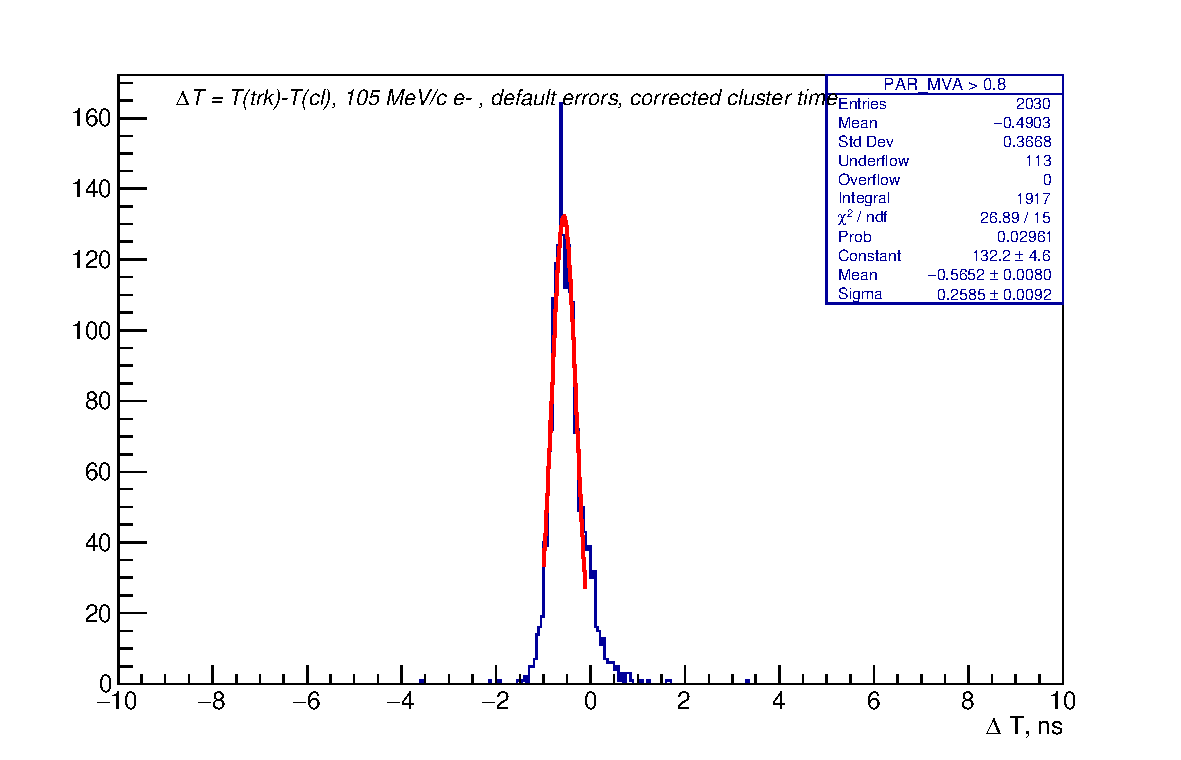
\includegraphics[width=0.64\textwidth]{figures/pdf/figure_00139_ele00s51b0_pid_emuana_trk_101_dt}
      % }
    };
    \node [text width=1cm, scale=0.8] at (13.7,-2) {(d)};
    % \node [text width=6cm, scale=0.8] at (4.5,6.4) {mu2e-18894 by Kevin Lynch and Jim Popp};
  \end{tikzpicture}
  % \captionof{figure} {
  \caption{
    \label{fig:track_cluster_dt}
    Track-cluster timing offsets and their correction: 
    (a) default offline configuration;
    (b) cluster assigned large errors in the fit; 
    (c) cluster timing corrected by 1.6 ns, still large errors;
    (d) cluster timing corrected by 1.6ns, default errors
  }
\end{figure}



%%% Local Variables:
%%% TeX-master: "mu2e-36375"
%%% End:

%%% -*- mode:latex; mode:flyspell -*-

%%% Local Variables:
%%% TeX-master: "mu2e-36575"
%%% End:
\section{Tuning the calorimeter timing resolution}

The calorimeter timing simulation has been significantly improved since the Offline version
v9\_0\_5 used to start SU2020 branch.
The old timing simulation was largely underestimating the calorimeter timing resolution.
A better parametrization of the photon propagation time inside the crystal and, most significantly, a better implementation of the noise in the simulation in more recent versions of the Offline produces  simulation results much closer to the test beam measurements \cite{MU2E_35540_CALO_TIMING}.

The different components of the calorimeter noise during the first period of data taking have been estimated in \cite{MU2E_35519_CALO_NOISE} 
assuming the Run Plan reported in \cite{MU2E_33731_RUN1_PLAN}, where the results are summarized
in Table \ref{table:calonoise}. 
The noise components include the electronic noise (measured at the cosmic ray stand), 
radiation induced noise (RIN), and dark current due to neutron radiation damage
in the SiPMs (assuming an operation temperature of $-10^o$ C).
A safety factor of 2 has been used for the  neutron induced noise to reflect the uncertainty of the results of neutron radiation damage measurements.

\begin{table}[htbp]
  \begin{center} 
    \begin{tabular}{|c|c|c|c|c|c|}
      \hline
      Run 1 period      & FEE noise  & RIN     & Dark current noise & RIN$\oplus$Dark   & FEE$\oplus$RIN$\oplus$Dark \\ 
      \hline
      1 batch start     & 200 keV    & 280 keV &  --                & 280 keV & 344 keV  \\
      1 batch end       & 200 keV    & 280 keV &  450 keV           & 530 keV & 566 keV  \\
      2 batch end       & 200 keV    & 400 keV &  492 keV           & 634 keV & 664 keV \\
      \hline
    \end{tabular}
  \end{center}
  \caption{
  \label{table:calonoise}
    Calorimeter noise levels in different Run 1 periods as estimated in \cite{MU2E_35519_CALO_NOISE}. 
  }
  % \vspace{0.5in}
\end{table}

A parametrization of the time resolution as function of the RIN$\oplus$Dark noise level (assuming FEE noise fixed at 200 keV) and the energy deposited
in a crystal obtained using the latest calorimeter simulation software has been presented in  \cite{MU2E_36225_CALO_TIME_RES}.

Using the results in the Table \ref{table:calonoise}, we assume an average RIN$\oplus$Dark noise of 405 keV for the 1 batch period and 580 keV for the 2 batch period. 
The curves obtained using Bertrand's parametrization are the lower dashed
lines in Figures \ref{fig:calorimeter_timing_resolution_1batch} and  \ref{fig:calorimeter_timing_resolution_2batch}.

Table \ref{table:calonoise} does not include the time jitter of the accelerator signal.
This effect should also be included in the tracker timing simulation, where it is currently
ignored. For particle identification, the only relevant quantity is the relative time
between the tracker and calorimeter. 
We decided not to change the tracker timing simulation, but instead to add the accelerator
clock jitter only to the cluster time.
Preliminary measurements \cite{MU2E_35392_TIME_JITTER} show a time jitter of 172 ps
for a chain of 2 DTCs and 217 ps for a chain of 7 DTCs. We take 200 ps as our best estimate.

Integration of the latest updates to the calorimeter simulation software into the SU2020 branch
would be a task, very complicated technically. Instead, an additional Gaussian time smearing
component is added to the  CaloCrystalHitFromHit module to reproduce the desired time resolution. 

Figures \ref{fig:calorimeter_timing_resolution_1batch} and  \ref{fig:calorimeter_timing_resolution_2batch} show the output of the time resolution
simulation with the additional Gaussian smearing component as a function of the energy deposited
in the crystal for the two calorimeter disks for 1 and 2 batch modes.
The agreement with the expected analytical function is shown. 
The deviations at small energies are not important as the time resolution simulation
in those regions is known to be less reliable.

\begin{figure}[h]
  \hspace{-0.6in}
  \begin{tikzpicture}
    \node[anchor=south west,inner sep=0] at (0.,0.) {
      % \node[shift={(0 cm,0.cm)},inner sep=0,rotate={90}] at (0,0) {}
      \makebox[\textwidth][c] {
        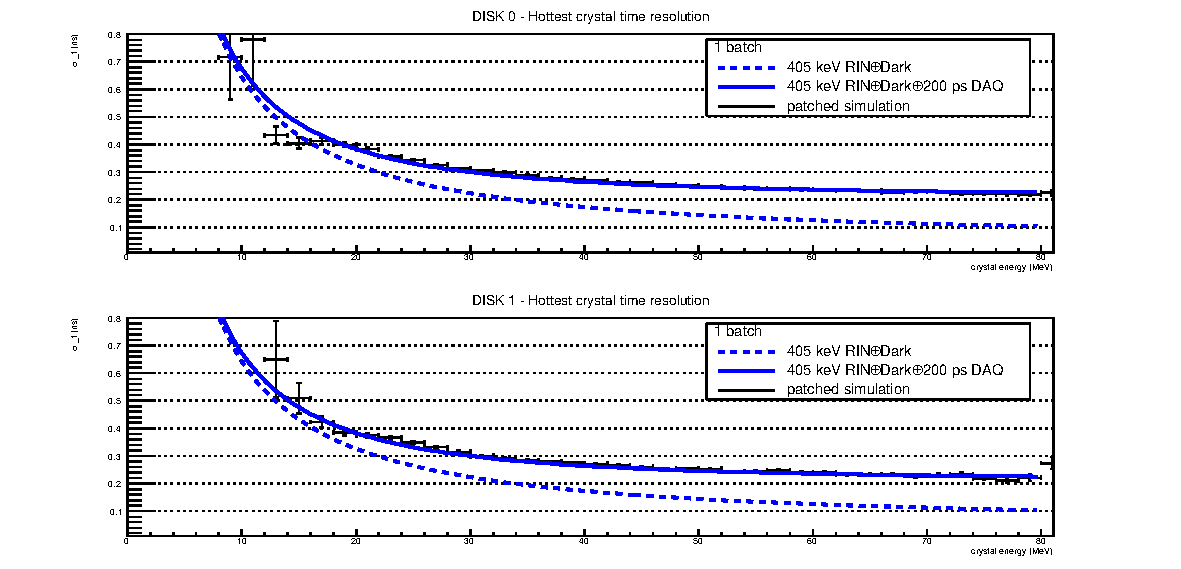
\includegraphics[width=0.70\textwidth, trim = 40 0 125 0]{figures/pdf/figure_00401_sigmat_1batch_corrected}
      }
    };
    % \node [text width=6cm, scale=0.8] at (4.5,6.4) {mu2e-18894 by Kevin Lynch and Jim Popp};
  \end{tikzpicture}
  % \captionof{figure} {
  \caption{
    \label{fig:calorimeter_timing_resolution_1batch}
    Tuning of the calorimeter timing resolution for the 1 batch run period.
    The lower dashed curve corresponds to the parametrization given in 
    \cite{MU2E_36225_CALO_TIME_RES} using a noise of 455 keV.
    The upper dashed curve includes the 200 ps for the DTCs time jitter.
    The black points represent the results of the SU2020 patched calorimeter time simulation.
  }
\end{figure}

\begin{figure}[h]
  \hspace{-0.6in}
  \begin{tikzpicture}
    \node[anchor=south west,inner sep=0] at (0.,0.) {
      % \node[shift={(0 cm,0.cm)},inner sep=0,rotate={90}] at (0,0) {}
      \makebox[\textwidth][c] {
        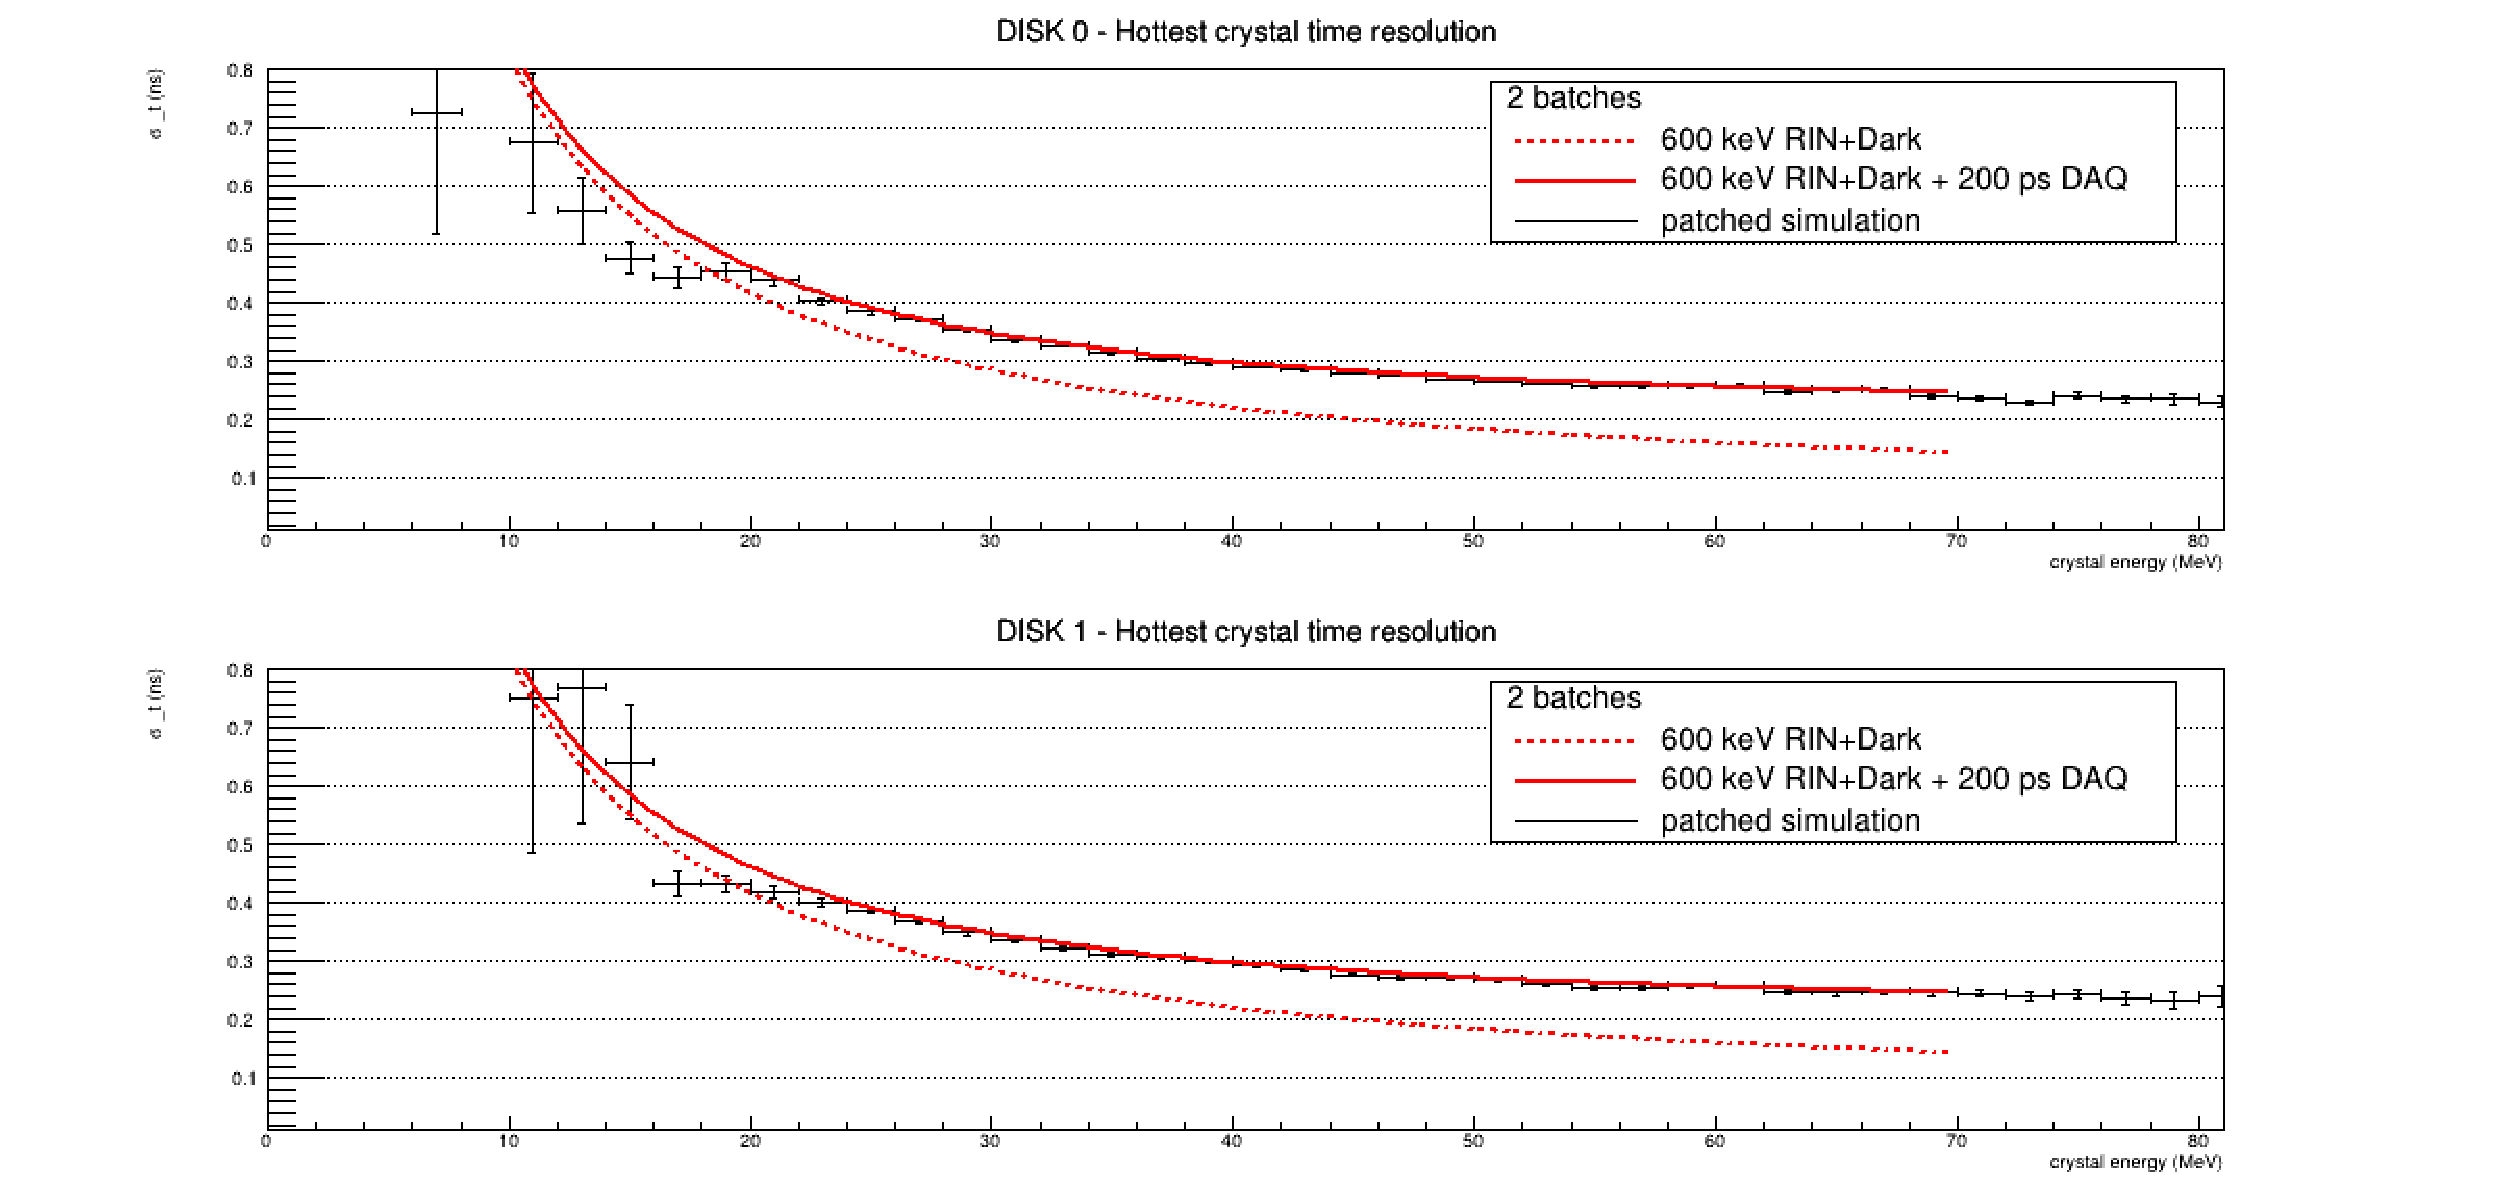
\includegraphics[width=0.70\textwidth, trim = 40 0 125 0]{figures/pdf/figure_00402_sigmat_2batch_corrected}
      }
    };
    % \node [text width=6cm, scale=0.8] at (4.5,6.4) {mu2e-18894 by Kevin Lynch and Jim Popp};
  \end{tikzpicture}
  % \captionof{figure} {
  \caption{
    \label{fig:calorimeter_timing_resolution_2batch}
    Tuning of the calorimeter timing resolution for the 2 batch run period.
    The lower dashed curve corresponds to the parametrization
    given in \cite{MU2E_36225_CALO_TIME_RES} using a noise of 600 keV.
    The upper dashed curve includes the 200 ps for the DTCs time jitter.
    The black points represent the results of the SU2020 patched calorimeter time simulation. 
  }
\end{figure}

%%% mode: latex; mode:flyspell
%%%%%%%%%%%%%%%%%%%%%%%%%%%%%%%%%%%%%%%%%%%%%%%%%%%%%%%%%%%%%%%%%%%%%%%%%%%%% 
\section{Track momentum corrections}

The mean value of the reconstructed track momentum extrapolated to the tracker entrance is
slightly lower than the true MC momentum of the corresponding MC particle.
The offset is of the order of 30 keV/c and slightly different the track fits with different
ambiguity resolvers. 
We correct the reconstructed momenta of PAR tracks by 34 keV/c , and DAR tracks - by 30 keV/c.

\begin{figure}[h]
\hspace{-0.6in}
\begin{tikzpicture}
  \node[anchor=south west,inner sep=0] at (0,0.) {
    % \node[shift={(0 cm,0.cm)},inner sep=0,rotate={90}] at (0,0) {}
    % \makebox[\textwidth][c] {
      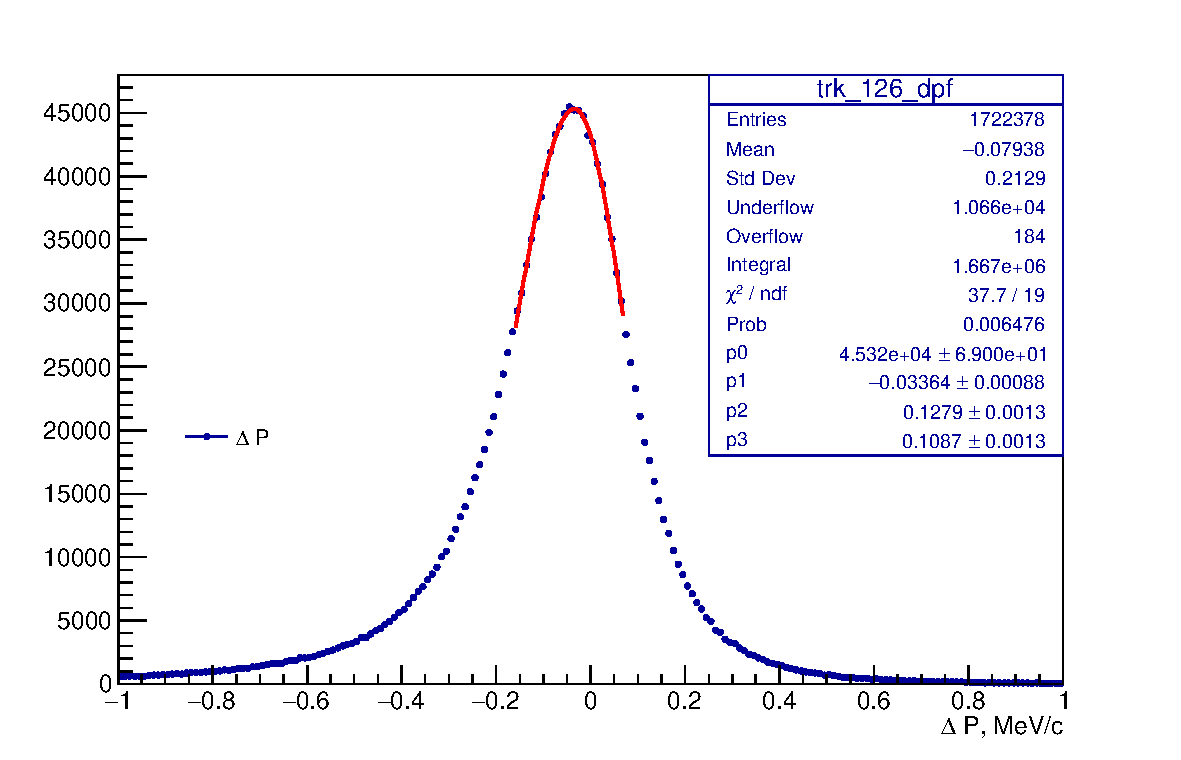
\includegraphics[width=0.65\textwidth]{figures/pdf/figure_00112_fele2s51b1_track_comp_ffff_1070_nocorr_trk_126_dpf}
    %}
  };
  \node[anchor=south west,inner sep=0] at (10,0.) {
    % \node[shift={(0 cm,0.cm)},inner sep=0,rotate={90}] at (0,0) {}
    % \makebox[\textwidth][c] {
      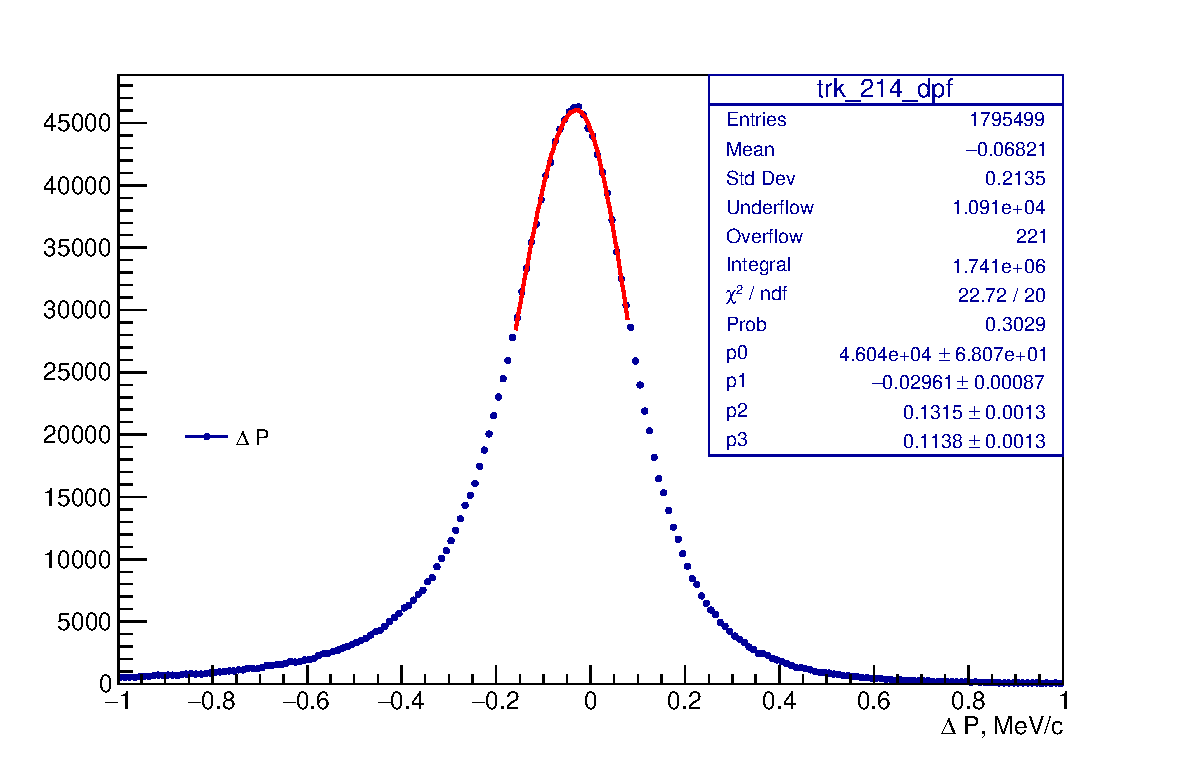
\includegraphics[width=0.65\textwidth]{figures/pdf/figure_00113_fele2s51b1_track_comp_ffff_1070_nocorr_trk_214_dpf}
    %}
  };
  % \node [text width=6cm, scale=0.8] at (4.5,6.4) {mu2e-18894 by Kevin Lynch and Jim Popp};
\end{tikzpicture}

\caption{
  \label{fig:sindrum_ii_fig_08_fit} 
  $\Delta P$ distributions at the tracker front for PAR (left) and DAR (right) tracks. The distributions  
  are fit with the asymmetric ($\sigma_{left} \ne \sigma_{right}$) gaussian function. Peak positions are used
  to correct the reconstructed  momenta of the tracks coming of the respective fits.
}
\end{figure}


%%% Local Variables:
%%% TeX-master: "mu2e-36575"
%%% End:

%%% Local Variables:
%%% mode: latex
%%% TeX-master: "mu2e-36575"
%%% End:

%%%%%%%%%%%%%%%%%%%%%%%%%%%%%%%%%%%%%%%%%%%%%%%%%%%%%%%%%%%%%%%%%%%%%%%%%%%%% 
\section{Track Selections}

Selection of correctly reconstructed tracks plays a critical role in the search.
In the Mu2e offline, there are two track fitters which correspond to two different
hit ambiguity resolvers. An ANN-based training has been performed only for one of them,
so-called ``panel-based ambiguity resolver''.

We performed a similar training for the output of the track fits using the doublet-based
ambiguity resolver.

Following \cite{MU2E_4595_ANN_TRAINING}, we used ROOT TMVA package to train a MLP ANN
with 8 input variables and one hidden layer. The following variables were used as inputs:

.....

The goal of training was to optimize separation of the electron tracks reconstructed correctly,
with $\Delta{P} = |P_{reco}-P_{true}| < 0.25$ MeV/c, or approximately $2\sigma$, from tracks
reconstructed with $\Delta{P} > 0.7$ MeV/c, or , approximately, $5\sigma$ above the true value.
The comparison between the $P_{true}$ and $P_{reco}$ was performed in a plane corresponding to
the tracker entrance. 

As a cross-check, we also trained a BDT-based TMVA classifier. Similar to \cite{MU2E_33150_ANN_TRAINING},
we found that the ANN performed slightly better, so current analysis uses an ANN-based track
quality selection.

\begin{figure}
\begin{tikzpicture}
  \node[anchor=south west,inner sep=0] at (0,0.) {
    % \node[shift={(0 cm,0.cm)},inner sep=0,rotate={90}] at (0,0) {}
    % \makebox[\textwidth][c] {
      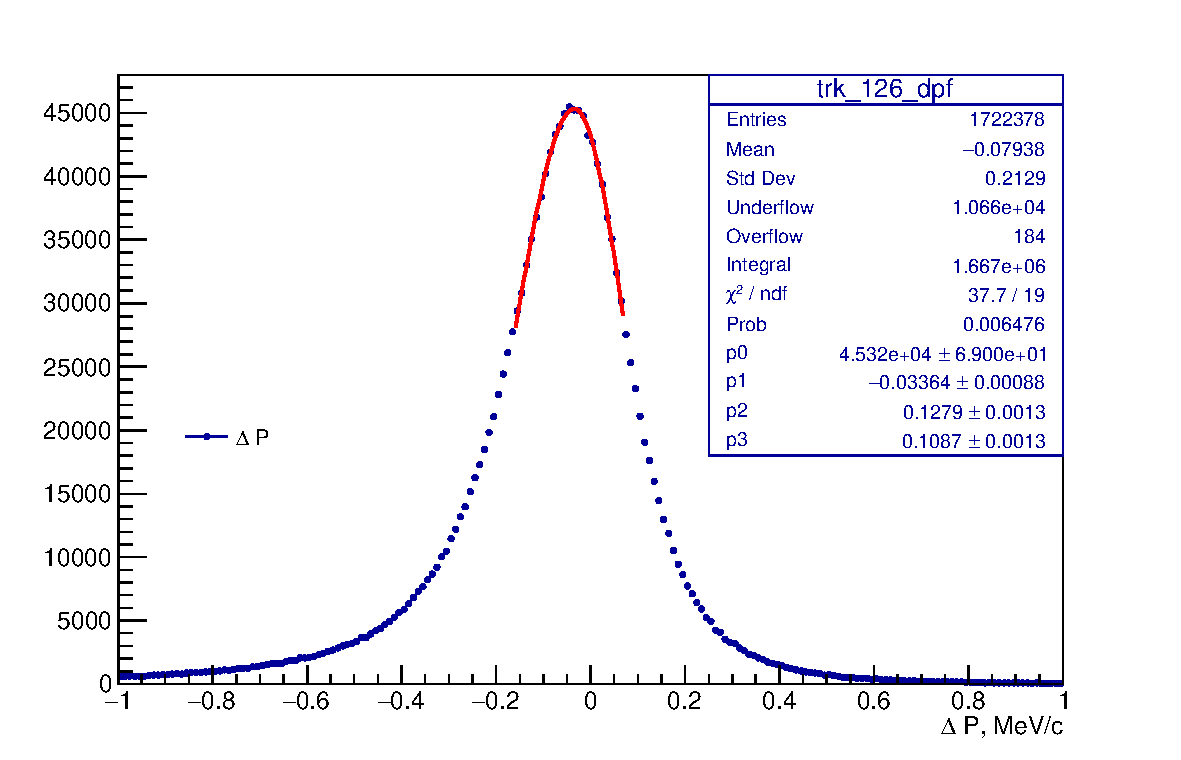
\includegraphics[width=0.55\textwidth]{figures/pdf/figure_00112_fele2s51b1_track_comp_ffff_1070_nocorr_trk_126_dpf}
    %}
  };
  \node[anchor=south west,inner sep=0] at (8,0.) {
    % \node[shift={(0 cm,0.cm)},inner sep=0,rotate={90}] at (0,0) {}
    % \makebox[\textwidth][c] {
      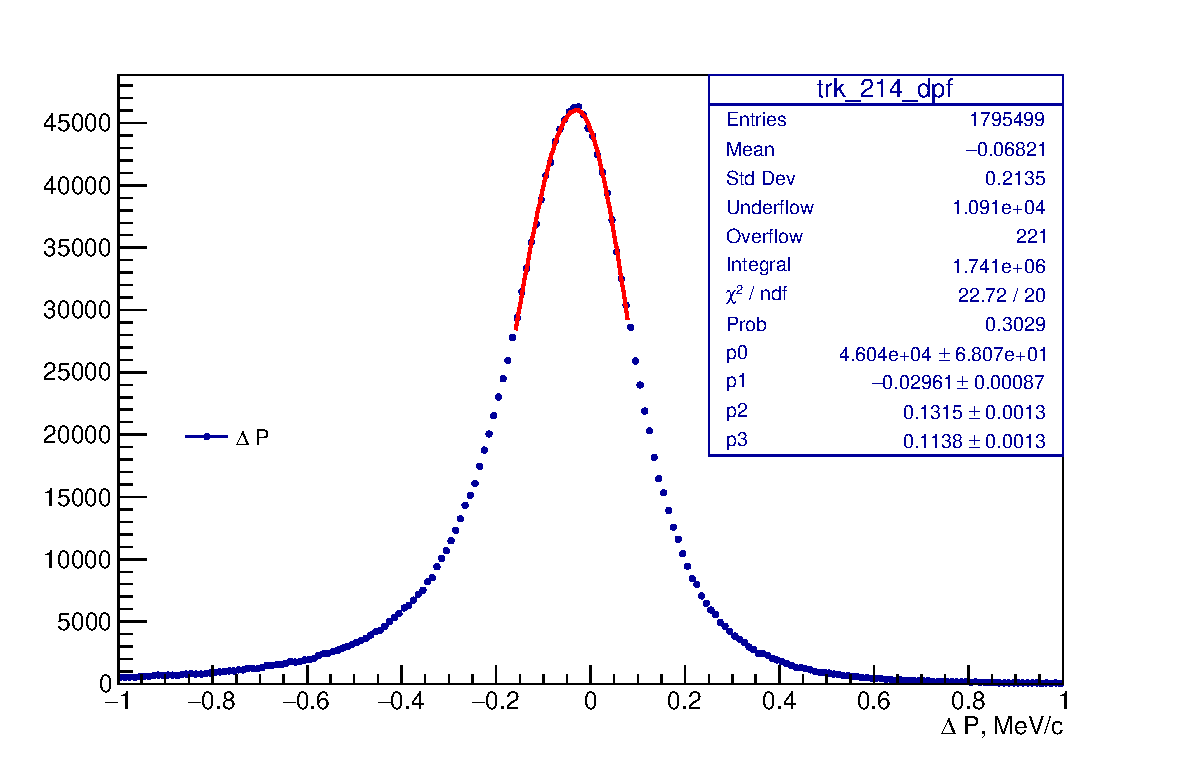
\includegraphics[width=0.55\textwidth]{figures/pdf/figure_00113_fele2s51b1_track_comp_ffff_1070_nocorr_trk_214_dpf}
    %}
  };
  % \node [text width=6cm, scale=0.8] at (4.5,6.4) {mu2e-18894 by Kevin Lynch and Jim Popp};
\end{tikzpicture}

\caption{
  \label{fig:sindrum_ii_fig_08_fit} 
  $\Delta P$ distributions at the tracker front for PAR (left) and DAR (right) tracks. The distributions  
  are fit with the asymmetric ($\sigma_{left} \ne \sigma_{right}$) gaussian function. Peak positions are used
  to correct the reconstructed  momenta of the tracks coming of the respective fits.
}
\end{figure}


Improvements in the track reconstruction resulted in a significantly better separation
between the two classes of tracks. For example, the expected relative contribution of
the DIO tracks with $\Delta{P} > 0.5$ MeV inthe ``signal'' region, [103.6,105.0] MeV/s was
found to be 0.228. This number is 50\% lower than 0.355, estimated in \cite{MU2E_4595_ANN_TRAINING}
for the same region.
\begin{figure}
\begin{tikzpicture}
  \node[anchor=south west,inner sep=0] at (0,0.) {
    % \node[shift={(0 cm,0.cm)},inner sep=0,rotate={90}] at (0,0) {}
    \makebox[\textwidth][c] {
      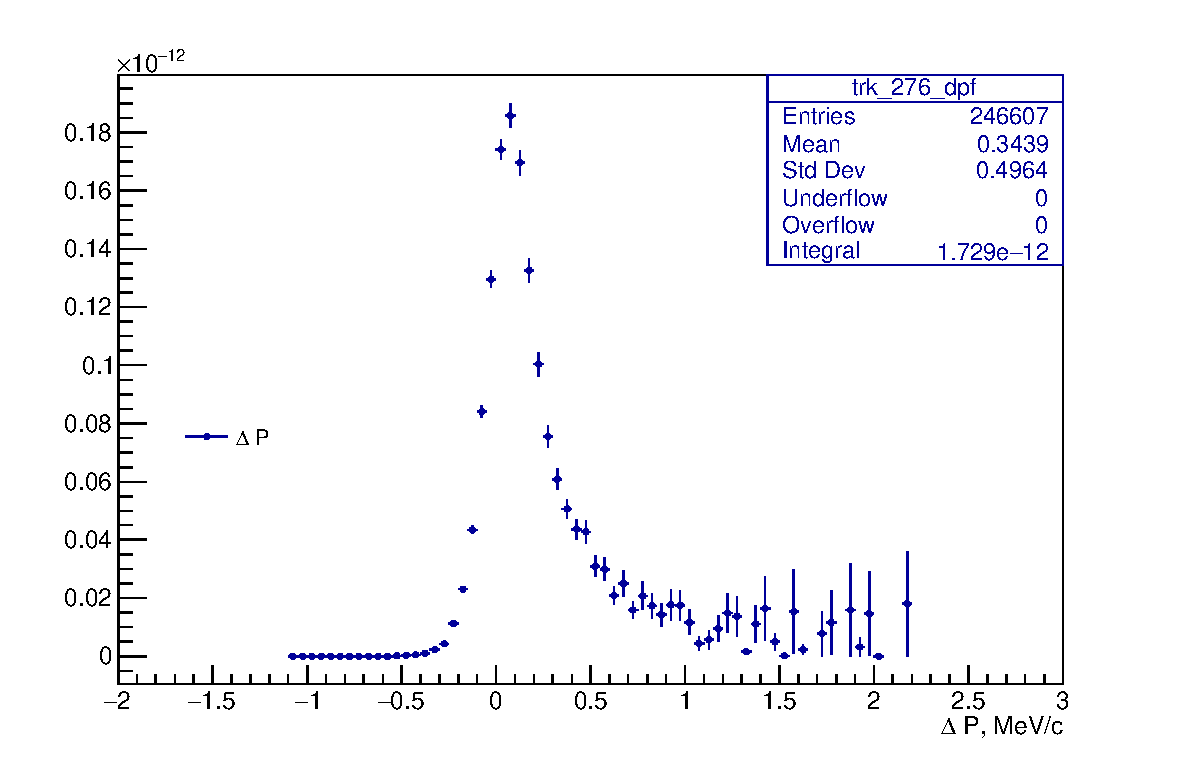
\includegraphics[width=0.99\textwidth]{figures/pdf/figure_00111_fele2s51b1_track_comp_ffff_1070_trk_276_dpf}
    }
  };
  % \node [text width=6cm, scale=0.8] at (4.5,6.4) {mu2e-18894 by Kevin Lynch and Jim Popp};
\end{tikzpicture}
% \captionof{figure} {
\caption{
  \label{fig:sindrum_ii_fig_08_fit} 
  $\Delta P ~=~ P_{reco} -P_{true}$ distribution for simulated DIO background in the region [103.6,105.0] MeV.
  77.2\% of reconstructed events in this region are expected to have $\Delta P < 0.5$ MeV/c
}
\end{figure}

To explore the parameter space, we also trained a similar ANN to discriminate the tracks for
$\Delta{P} < 0.25$ MeV/c from tracks with $\Delta{P} > 0.6$ MeV/c. No improvement in the DIO
suppression in the region [103.85, 104.9] MeV/c was observed. 

To choose between the PAR-based and DAR-based fitters, we compared performance of the
trained DAR ANN to the performance of the PAR ANN.

The results are shown in Figure ..... .
Using the CD3 choice of the signal region , 103.85 < p < 104.9 MeV/c, we compared the
CE reconstruction efficiency of the two methods vs the expected DIO background.

The relative efficiency is 
% -*- mode: latex; mode: flyspell -*-

%%% Local Variables:
%%% TeX-master: "mu2e-36575"
%%% End:

%%%%%%%%%%%%%%%%%%%%%%%%%%%%%%%%%%%%%%%%%%%%%%%%%%%%%%%%%%%%%%%%%%%%%%%%%%%%%%
\section{Particle identification}
% {\blue lowercase title words after first word}

For muons, the momentum region around 100 MeV/c for muons the region where the transition 
the non-relativistic to the ultra-relativistic regime is happening.
As shown in Figure \ref{fig:pid_ep_dt}, distributions of important particle ID variables 
for 92 MeV/c and 105 MeV/c muons are quite different. Therefore it makes sense to optimize
the particle ID algorithms for the \MuToEm\ and \MuToEp\ conversion searches separately.

\begin{figure}[H]
\hspace{-0.6in}
  \begin{tikzpicture}
    \node[anchor=south west,inner sep=0] at (0,0.) {
      % \node[shift={(0 cm,0.cm)},inner sep=0,rotate={90}] at (0,0) {}
      % \makebox[\textwidth][c] {
      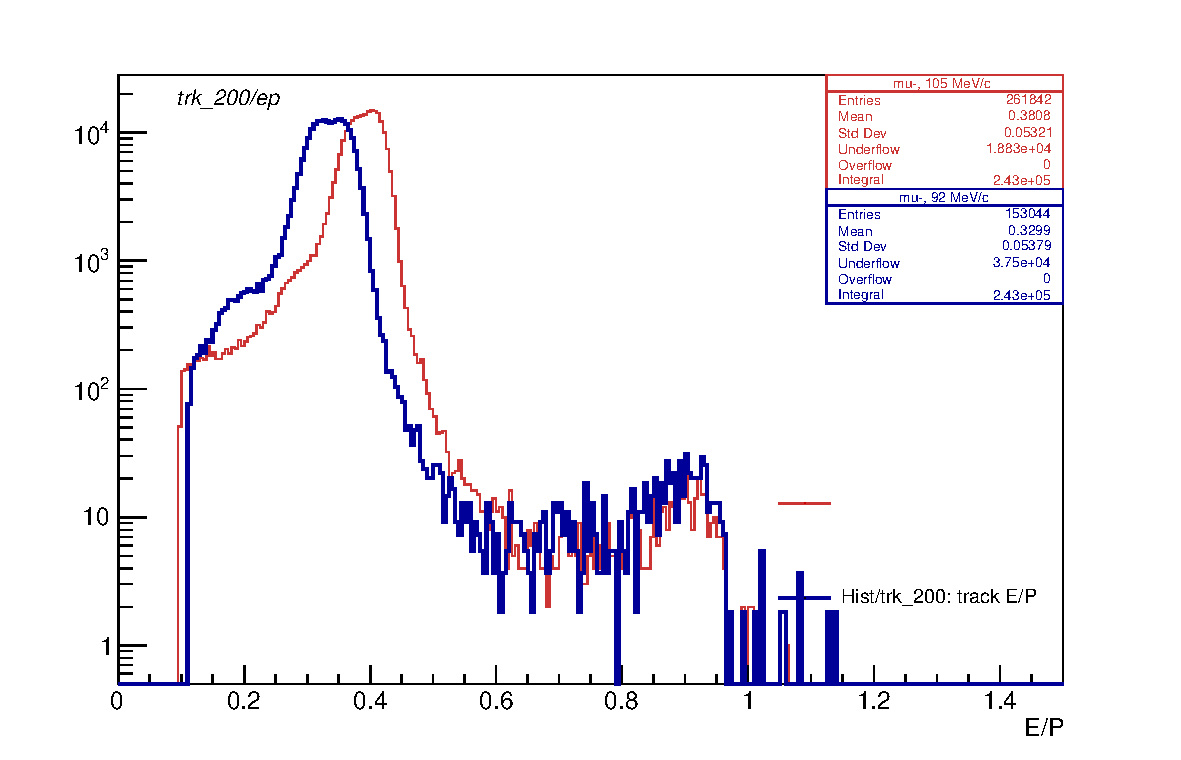
\includegraphics[width=0.64\textwidth]{figures/pdf/figure_00321_su2020_track_ana_trk_200_ep}
      % }
    };
    \node[anchor=south west,inner sep=0] at (10.5,0.) {
      % \node[shift={(0 cm,0.cm)},inner sep=0,rotate={90}] at (0,0) {}
      % \makebox[\textwidth][c] {
      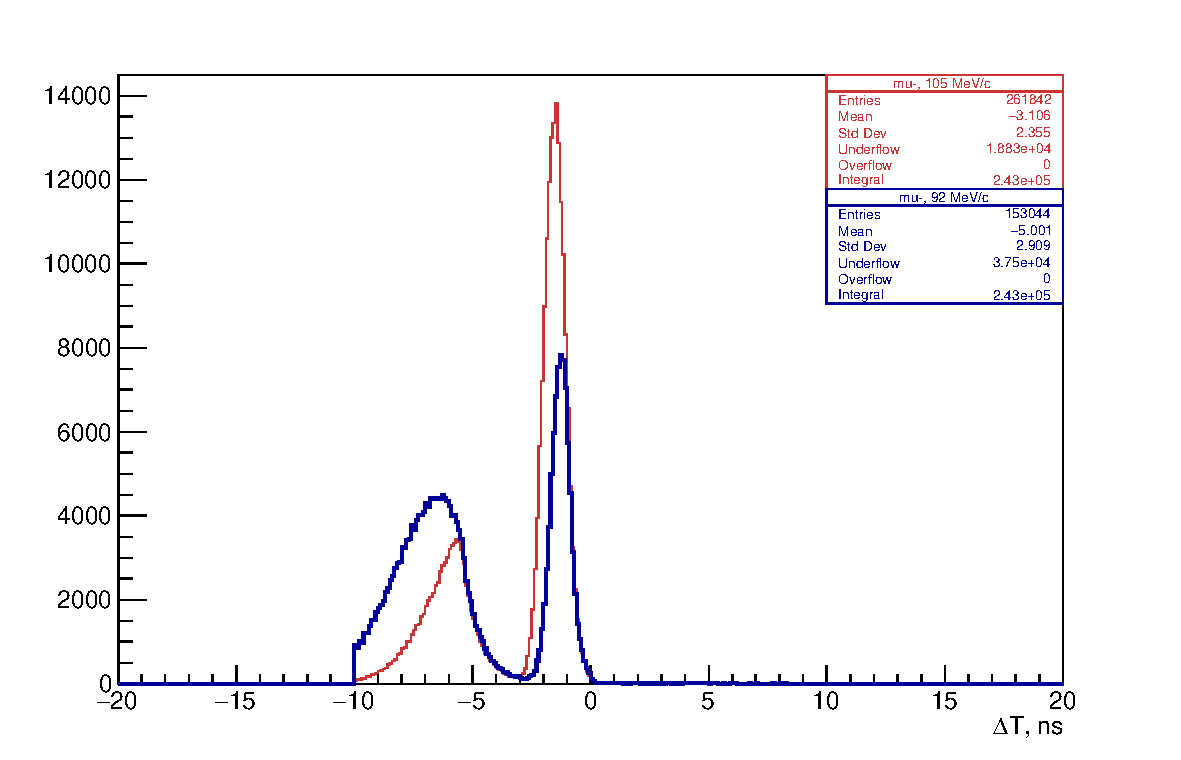
\includegraphics[width=0.64\textwidth]{figures/pdf/figure_00322_su2020_track_ana_trk_200_dt}
      % }
    };
    % \node [text width=6cm, scale=0.8] at (4.5,6.4) {mu2e-18894 by Kevin Lynch and Jim Popp};
  \end{tikzpicture}
  % \captionof{figure} {
  \caption{
    \label{fig:pid_ep_dt}
    The E/P and $\Delta{T} = T_0 - T_{\rm cluster}$ distributions for 105 and 92 MeV/c muon tracks reconstructed under an
    electron hypothesis. The bump inbetween -10 and -5 ns in the $\Delta{T}$ distributions corresponds
    to events with the calorimeter cluster rejected by the track fit, so the track $T_0$ is not biased by the fit.
    Events in the peak around -1.5 ns have the cluster used by the fit and thus biasing the fit results.
  }
\end{figure}

There is an indication that the bias resulting from the inclusion of the calorimeter cluster
into the track fit somewhat degrades the separation between electrons and muons.
%
At the same time, inclusion of the cluster into the track fit stabilizes the track fit, improves its
convergence and, overall, results in a higher track reconstruction efficiency.
%
Taking both considerations into account, we have chosen to use ANN-based PID classifiers,
expecting the ANN training to ``absorb'' existing systematic effects while providing a sufficiently
high level of muon rejection.
Single particle datasets {\bf ele00s61b0} and {\bf mumi0s61b0},  105 MeV/c electrons and negative muons,
have been used to train the PID ANN for the \MuToEm\ channel.

%%%%%%%%%%%%%%%%%%%%%%%%%%%%%%%%%%%%%%%%%%%%%%%%%%%%%%%%%%%%%%%%%%%%%%%%%%%%%%
\subsection {PID ANN training }
\label{sec:mumem_pid_ann_training}
% {\blue lowercase title words after first word}

MVA classifiers were trained only for DAR tracks, however, based on the nature of 
the variables used, the trained MVA should perform equally well for PAR tracks.
%
Both electron and muon reconstruction were run on the same event. 
In principle, using information from two reconstruction passes on a given event adds information that may improve electron-muon separation.
However, it was found that adding  the requirement that each track is reconstructed under
an electron and muon hypotheses complicates reconstruction logic and increases
the number of special cases to consider without providing a visible improvement. 
Therefore, inputs for the ANN training are provided by the electron reconstruction only.

Events used for ANN training were required to have a downstream DAR track passing
the track selection cuts described in Section \ref{sec:track-selection_cuts_summary}.
%
The following event variables were used in the ANN training:

\begin{itemize}
\item 
  {\bf E(cluster)/P(track)} : although all tracks used in training have the same generated momentum,
  using E/P reduces dependence on the track momentum 
\item 
  {\bf N(crystals)} : the number of crystals in the reconstructed calorimeter cluster
\item 
  {\bf eSeedfr} : the fraction of energy in the seed crystal ($E_{seed}/E_{cluster}$)
\item 
  {$\bf \Delta T$} : the time residual of the calorimeter cluster as determined by the Kalman fit
\item 
  {$\bf Z_{cluster}$} : the cluster Z-coordinate (within the corresponding calorimeter disk) as determined by the Kalman fit
\item 
  {$\bf \Delta R$} : the radial residual of the calorimeter cluster as determined by the Kalman fit
\item 
  {\bf path} : the overall length of the trajectory within the calorimeter disk
\end{itemize}

The PID ANN training is performed using the ROOT TMVA package ; it uses 10000 electron and 10000 muon events.
Events with muon decays in flight are excluded from training by requiring the last point (StepPointMC)
of the muon MC trajectory to have Z > 10000 mm.
%
To ensure that all event variables used in the ANN training are defined, events used for training
are required to pass the following requirements:

\begin{itemize}
\item 
  the track reconstructed under electron hypothesis passes the $\MuToEm$ track selection cuts
\item 
  the event has a reconstructed cluster 
\item 
  $\Delta T > -100$ ns : this is a requirement for the calorimeter cluster not to be rejected by the track fit.
  If the cluster is rejected, the $\Delta T$ value is set to -999 ns.
\item
  $-50 mm ~<~ Z_{cluster} ~<~ 250 mm$ : after the fit, the cluster Z coordinate is consistent in Z with the
  Z-position of the corresponding calorimeter disk.
\end{itemize}

Figures \ref{fig:pid_training_1} and \ref{fig:pid_training_2} show the distributions of the electron
and muon variables used for the PID ANN training.

\begin{figure}[H]
  \hspace{-0.6in}
  \begin{tikzpicture}
    \node[anchor=south west,inner sep=0] at (-1,0.) {
      % \node[shift={(0 cm,0.cm)},inner sep=0,rotate={90}] at (0,0) {}
      % \makebox[\textwidth][c] {
      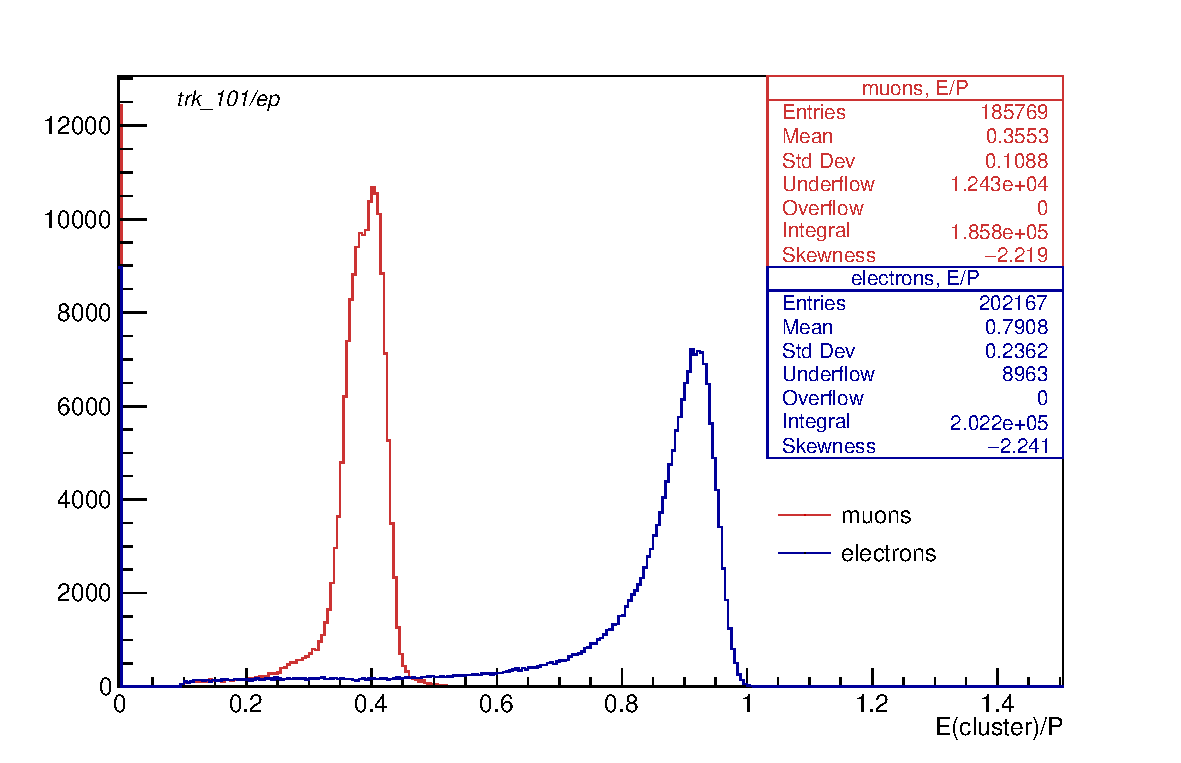
\includegraphics[width=0.50\textwidth]{figures/pdf/figure_00300_pid_emuana_1070_trk_101_ep}
    % }
    };
    \node[anchor=south west,inner sep=0] at (9.5,0.) {
      % \node[shift={(0 cm,0.cm)},inner sep=0,rotate={90}] at (0,0) {}
      % \makebox[\textwidth][c] {
      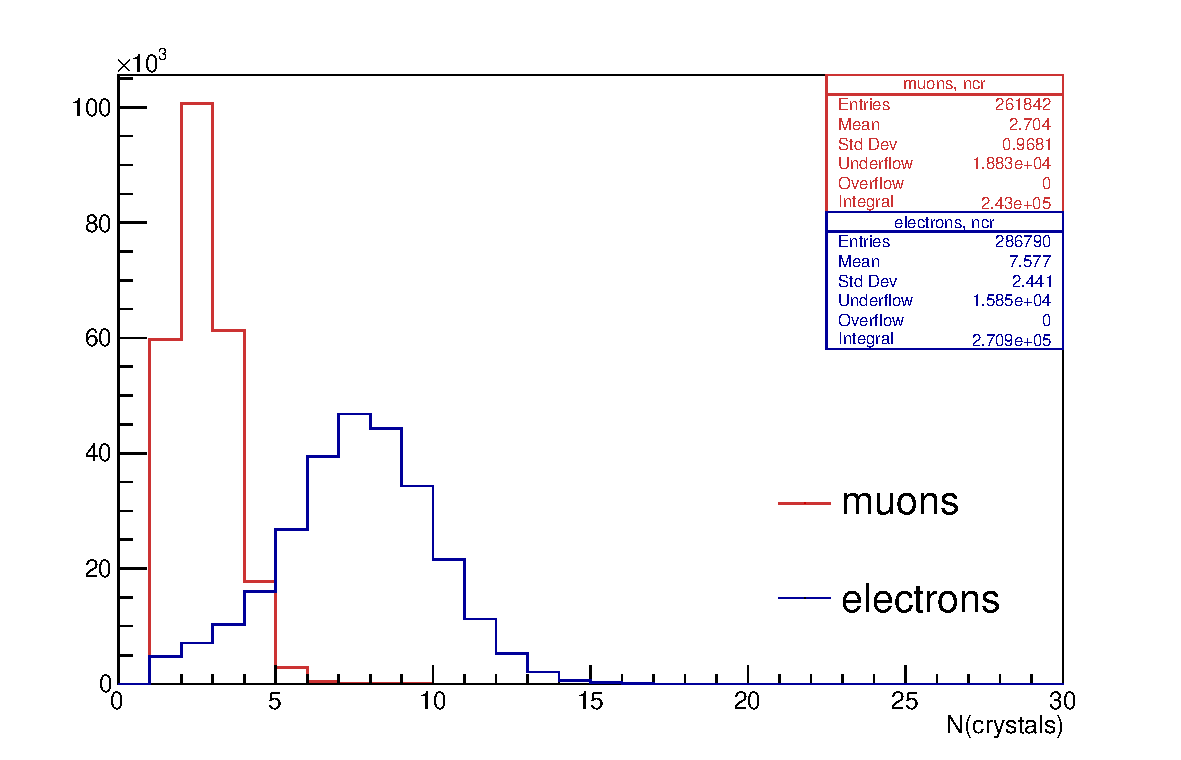
\includegraphics[width=0.50\textwidth]{figures/pdf/figure_00301_pid_emuana_1070_trk_101_ncr}
      % }
    };
    \node[anchor=south west,inner sep=0] at (-1,-6.) {
      % \node[shift={(0 cm,0.cm)},inner sep=0,rotate={90}] at (0,0) {}
      % \makebox[\textwidth][c] {
      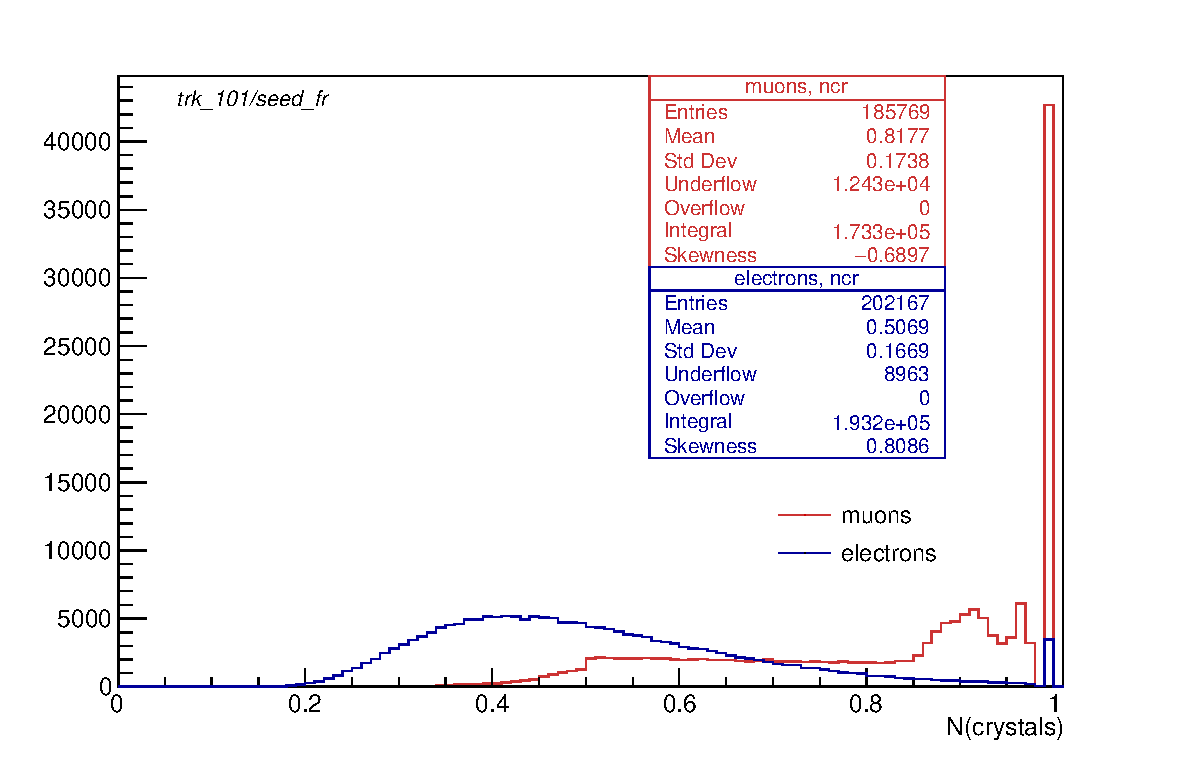
\includegraphics[width=0.50\textwidth]{figures/pdf/figure_00302_pid_emuana_1070_trk_101_seed_fr}
      % }
    };
    \node[anchor=south west,inner sep=0] at (9.5,-6.) {
      % \node[shift={(0 cm,0.cm)},inner sep=0,rotate={90}] at (0,0) {}
      % \makebox[\textwidth][c] {
      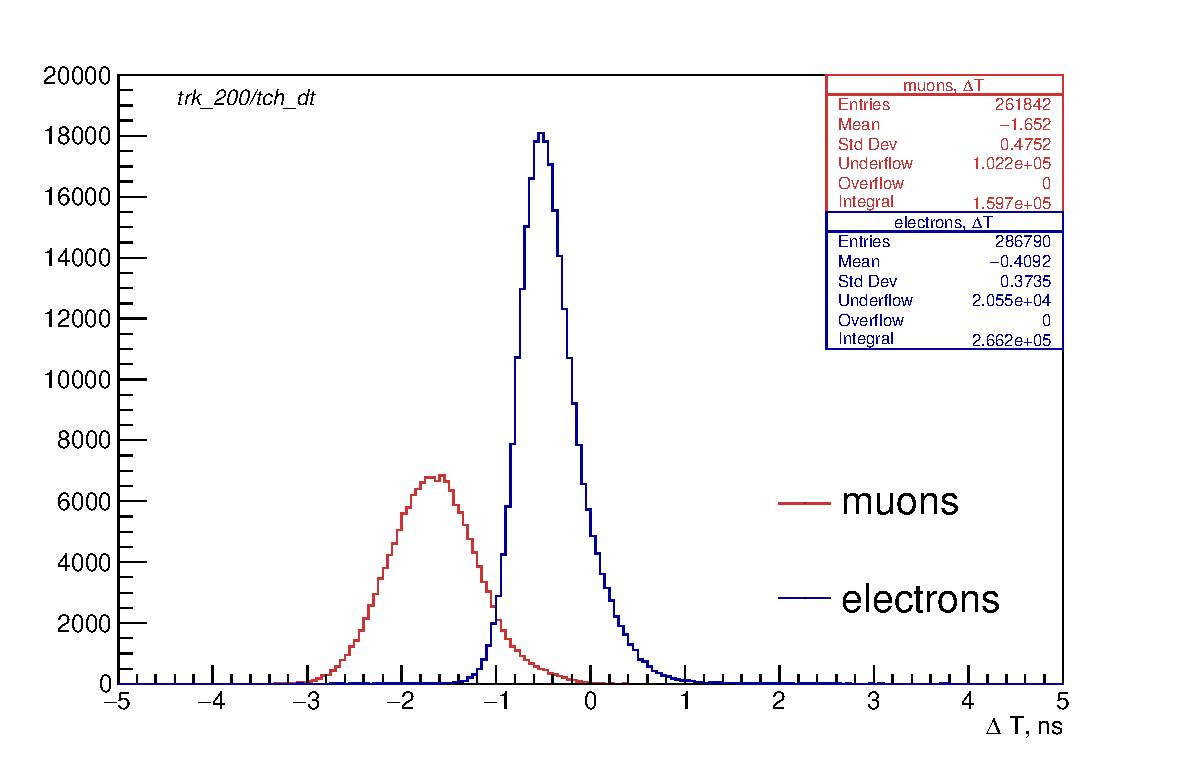
\includegraphics[width=0.50\textwidth]{figures/pdf/figure_00303_pid_emuana_1070_trk_101_tch_dt}
      % }
    };
    % \node [text width=6cm, scale=0.8] at (4.5,6.4) {mu2e-18894 by Kevin Lynch and Jim Popp};
  \end{tikzpicture}
  % \captionof{figure} {
  \caption{
    \label{fig:pid_training_1}
    The variables used in the PID ANN training: E/P, N(crystals), E(seed)/E, $\Delta T$
  }
\end{figure}

%%%%%%%%%% another figure
\begin{figure}[H]
  \hspace{-0.6in}
  \begin{tikzpicture}
    \node[anchor=south west,inner sep=0] at (0,0.) {
      % \node[shift={(0 cm,0.cm)},inner sep=0,rotate={90}] at (0,0) {}
      % \makebox[\textwidth][c] {
      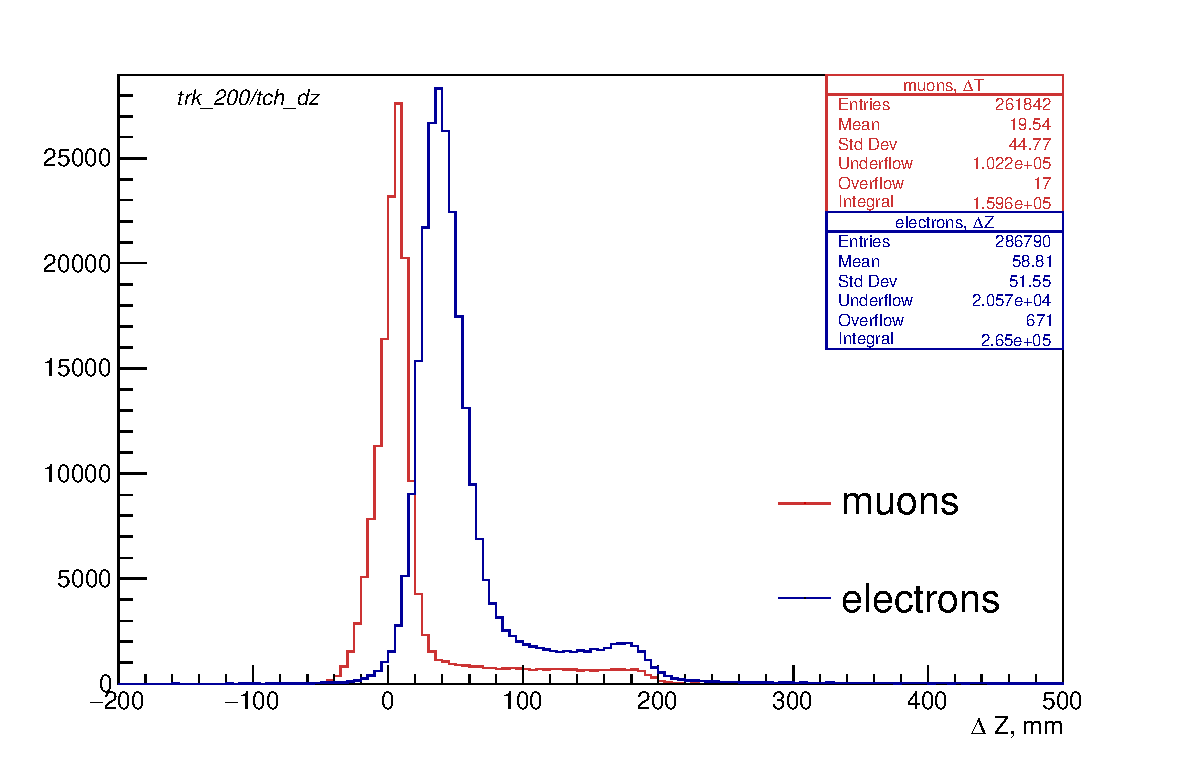
\includegraphics[width=0.50\textwidth]{figures/pdf/figure_00304_pid_emuana_1070_trk_101_tch_dz}
      % }
    };
    \node[anchor=south west,inner sep=0] at (10.5,0) {
      % \node[shift={(0 cm,0.cm)},inner sep=0,rotate={90}] at (0,0) {}
      % \makebox[\textwidth][c] {
      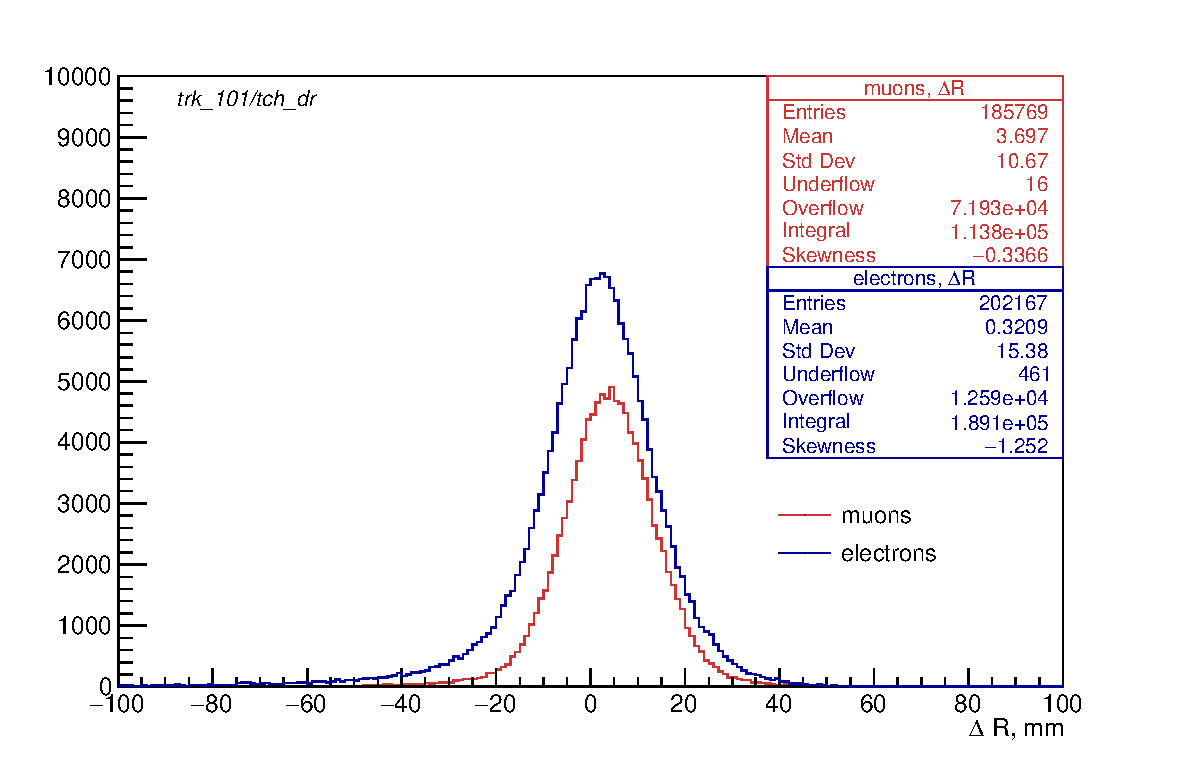
\includegraphics[width=0.50\textwidth]{figures/pdf/figure_00305_pid_emuana_1070_trk_101_tch_dr}
      % }
    };
    \node[anchor=south west,inner sep=0] at (0.,-6) {
      % \node[shift={(0 cm,0.cm)},inner sep=0,rotate={90}] at (0,0) {}
      % \makebox[\textwidth][c] {
      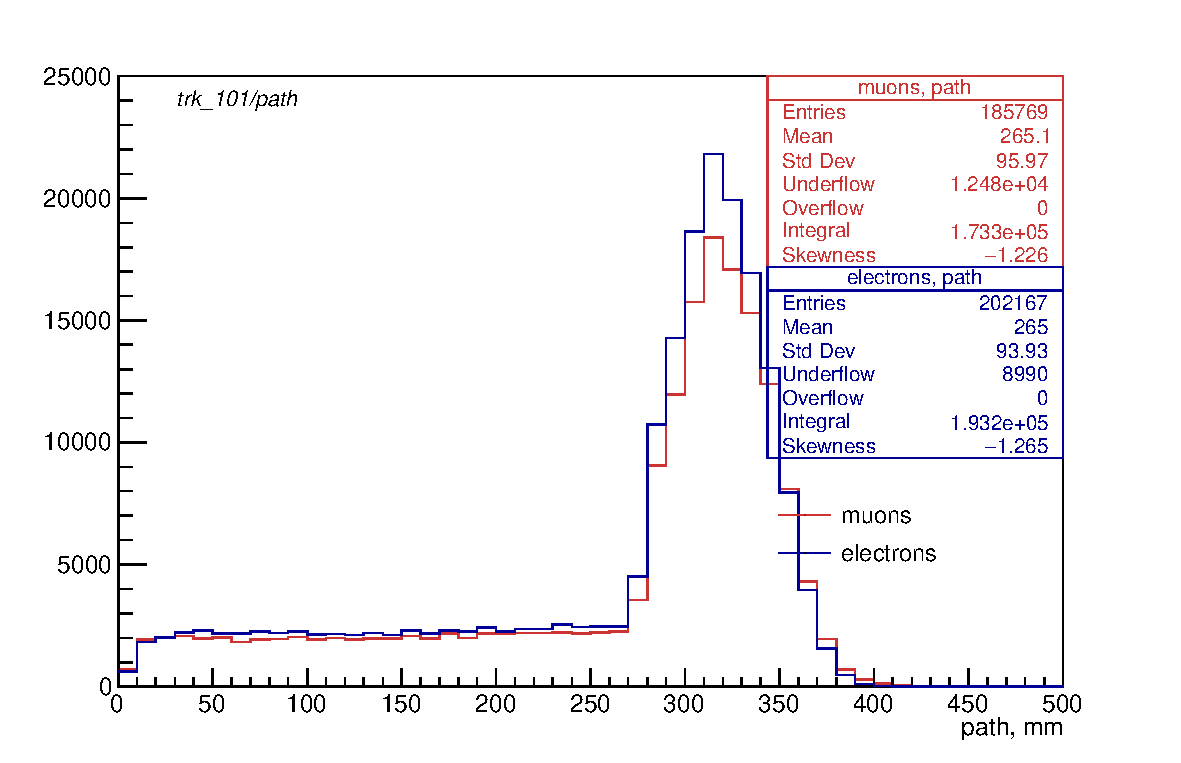
\includegraphics[width=0.50\textwidth]{figures/pdf/figure_00306_pid_emuana_1070_trk_101_path}
      % }
    };
    % \node [text width=6cm, scale=0.8] at (4.5,6.4) {mu2e-18894 by Kevin Lynch and Jim Popp};
  \end{tikzpicture}
  %% \captionof{figure} {
    \caption{
    \label{fig:pid_training_2}
    The variables used in the PID ANN training: $\Delta Z$, $\Delta R$, path
  }
\end{figure}


Results of the PID ANN training are shown in Figure \ref{fig:pid_training_3}. 
From the training plots, one might conclude that the separation between the
electrons and muons provided by the ANN is close to perfect. 
To identify 105 MeV electrons, we require the PID ANN score $S_{PID} > 0.5$.
The PID ANN training is validated by running the PID algorithm on the full ele00s61b0 and mumi0s51b0 datasets.
The datasets have about 200K events each, including events used for training.
The results presented in Figure \ref{fig:pid_training_4} show that the efficiency of a $S_{PID} > 0.5$ cut 
for electrons is about 99.2\%, and about 0.8\% of muons are mis-identified as electrons.
The spike at 1 in the ANN score distribution for muons corresponds to muon decays in flight,
where the particle reconstructed in the event is an electron.
Remaining sources of muon mis-identification will be studied in detail later.
To identify 105 MeV electrons for SU2020 analyses, we require a PID ANN score of $S_{PID} > 0.5$.


\begin{figure}[H]
\hspace{-0.6in}
  \begin{tikzpicture}
    \node[anchor=south west,inner sep=0] at (0,0.) {
      % \node[shift={(0 cm,0.cm)},inner sep=0,rotate={90}] at (0,0) {}
      % \makebox[\textwidth][c] {
      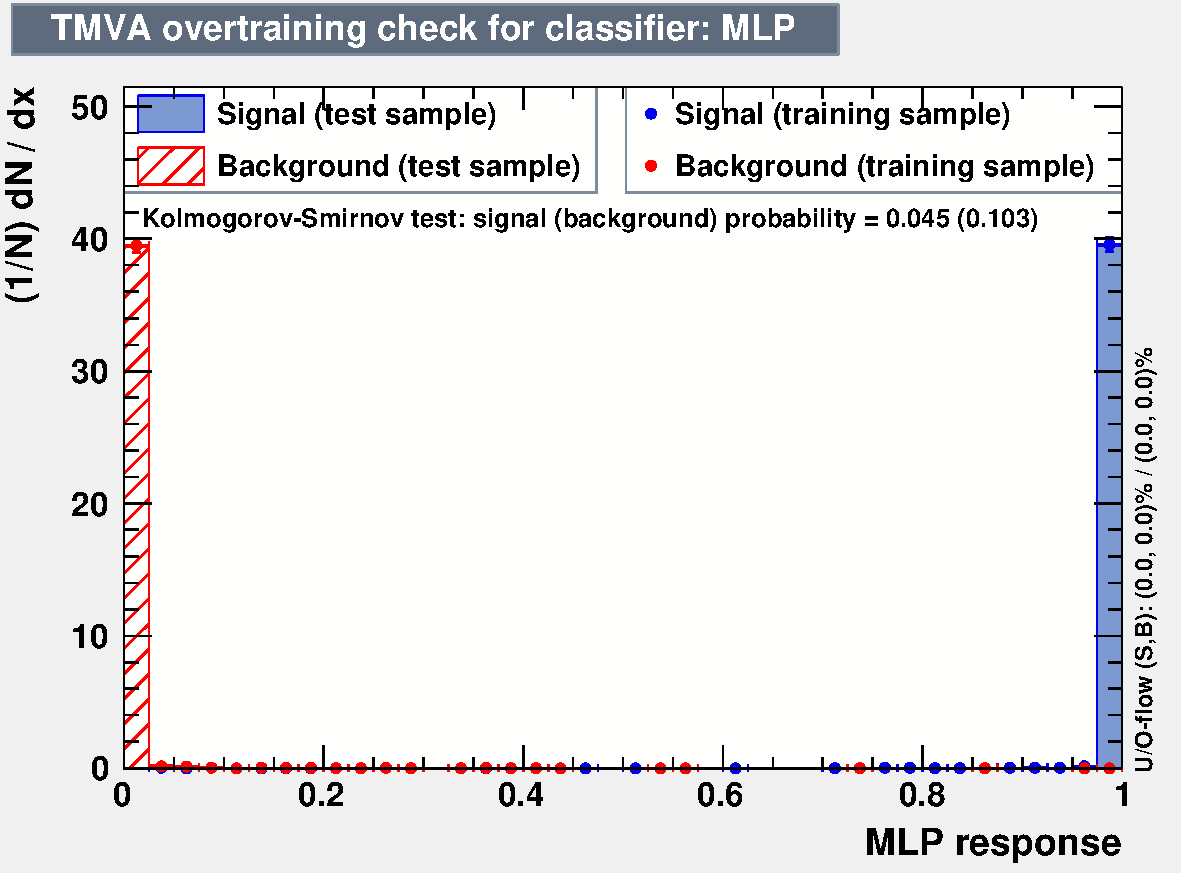
\includegraphics[width=0.55\textwidth]{figures/pdf/pid_mva_overtrain_mlp}
      % }
    };
    \node[anchor=south west,inner sep=0] at (10.5,0.5) {
      % \node[shift={(0 cm,0.cm)},inner sep=0,rotate={90}] at (0,0) {}
      % \makebox[\textwidth][c] {
      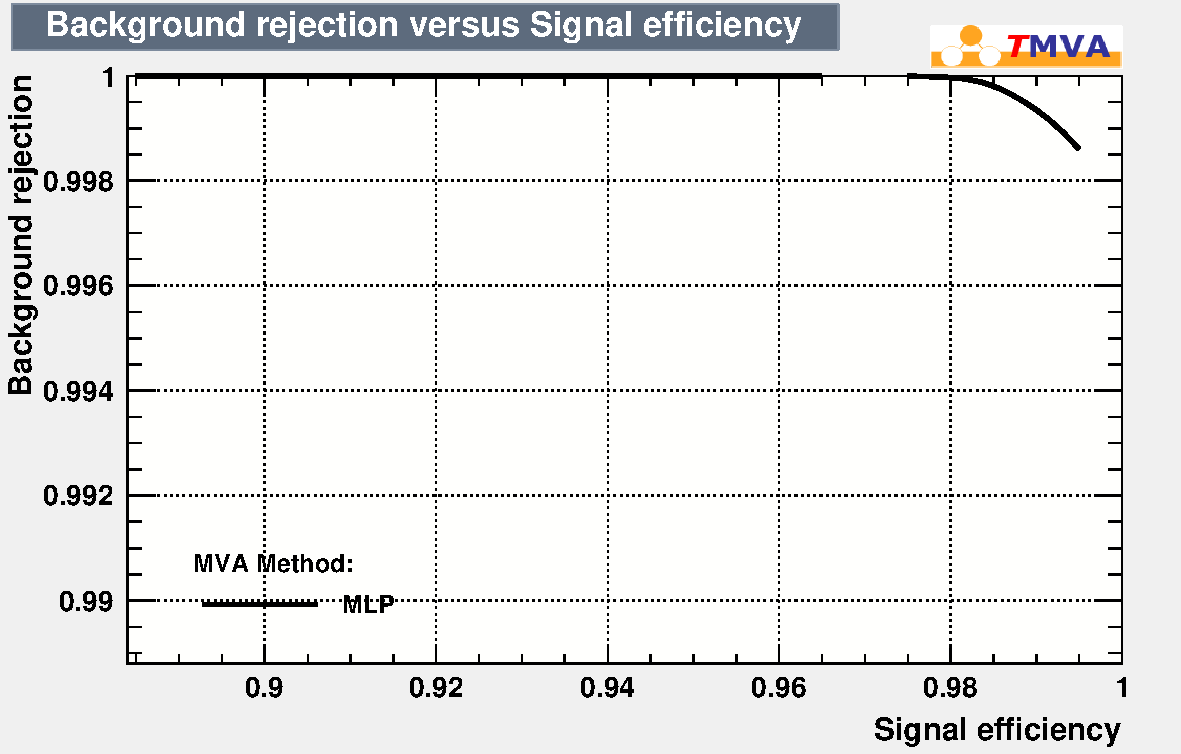
\includegraphics[width=0.55\textwidth]{figures/pdf/pid_mva_rejection_mlp}
      % }
    };
    % \node [text width=6cm, scale=0.8] at (4.5,6.4) {mu2e-18894 by Kevin Lynch and Jim Popp};
  \end{tikzpicture}
  % \captionof{figure} {
  \caption{
    \label{fig:pid_training_3}
    The output of the PID ANN training: overtraining check on the left and efficiency vs rejection 
    on the right
  }
\end{figure}

\begin{figure}[H]
  \begin{tikzpicture}
    \node[anchor=south west,inner sep=0] at (0,0.) {
      % \node[shift={(0 cm,0.cm)},inner sep=0,rotate={90}] at (0,0) {}
      \makebox[\textwidth][c] {
        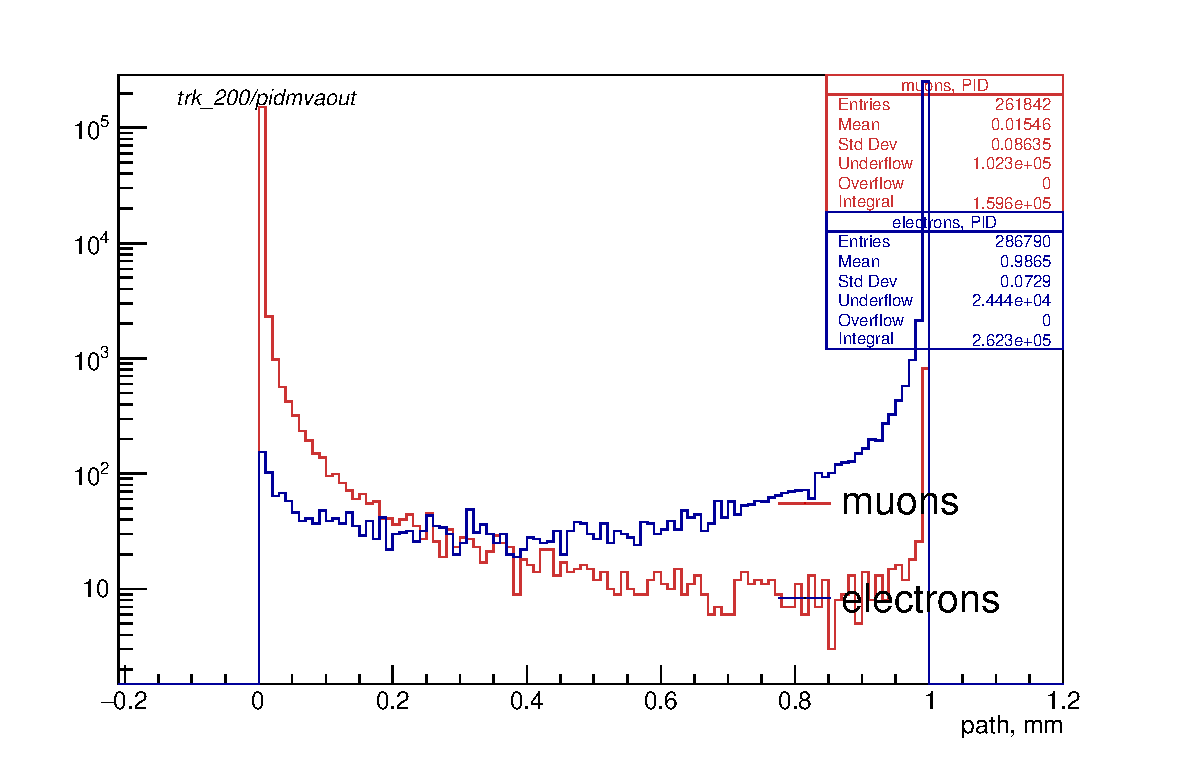
\includegraphics[width=1.0\textwidth]{figures/pdf/figure_00307_pid_emuana_1070_trk_101_pidmvaout}
      }
    };
    % \node [text width=6cm, scale=0.8] at (4.5,6.4) {mu2e-18894 by Kevin Lynch and Jim Popp};
  \end{tikzpicture}
  % \captionof{figure} {
  \caption{
    \label{fig:pid_training_4}
    Distribution in the PID ANN score for electron and muon samples, samples include events used for training,
    10000 events each. A spike in muon PID at 1  - muon decays in flight. \\ 
    % {\color{red} \bf check that underflows are events without clusters}
  }
\end{figure}

The efficiencies of the PID preselection cuts for the {\bf cele0s61b1} dataset are listed
in Table \ref{tab:pid_preselection_cuts}. The total preselection efficiency is about 93\%.
%
Out of that, approximately, 96\% comes from the requirement on the calorimeter cluster that E > 10 MeV
to be reconstructed in an event. Therefore, for events with the reconstructed track with $P > 100$ MeV/c 
and a reconstructed cluster, efficiency of the PID preselection is 96.7 \%

% Q: how does 96\% of the inefficiency come from the cluster requirement, but after this efficiency is still 96.7\%?.
% A: 0.96*0.967 = 0.93

For single track 105 MeV/c electron events passing the PID preselection, the efficiency
of the $S_{PID} > 0.5$ cut is 99.3\% .
\begin{table}[H]
  \begin{center}
    \begin{tabular}{l|c|c} % <-- Changed to S here.
      \textbf{Cut}                    & \textbf{N events after } & \textbf{Efficiency }\\
      \hline
      Number generated events         & 1000000                  &            \\
      total number of tracks          &  329715                  &   0.330    \\
      \hline                                                     
      track passes TID cuts           &  193252                  &   0.586    \\
      $P > 100$ MeV/c                 &  178078                  &   0.921    \\
      $|\Delta{T}| < 10$ ns           &  167028                  &   0.937     \\
      $-50 < dz < 250$                &  164951                  &   0.988    \\
      $ E/P < 1.2$                    &  164884                  &   1.000    \\
      \hline                                                     
      $S_{PID} >0.5$                   &  163543                  &   0.992    \\
   \end{tabular}
  \end{center}
  \caption{
    \label{tab:pid_preselection_cuts}
    The PID preselection cuts (defined using {\bf ele00s61b0} ) and the efficiency for {\bf cele0s51b1} electrons.
    TID cuts refers to the track ID cuts for the $\MuToEm$ channel.
    \\
    % {\red check which dataset the efficiencies are given for} 
  }
\end{table}

Out of 109004 muons with $P > 100$ MeV/c and passing the preselection cuts, 776 have a PID ANN score $S_{PID} > 0.5$,
which corresponds to a fake rate of about 0.7\%. Leading contributions to that rate come from muon decays in flight 
and decays of stopped muons in the calorimeter.

%%%%%%%%%%%%%%%%%%%%%%%%%%%%%%%%%%%%%%%%%%%%%%%%%%%%%%%%%%%%%%%%%%%%%%%%%%%%%%
\subsection { Electrons failing the PID selection}
\label{sec:electrons_failing_pid}

Figure \ref{fig:electrons_failing_pid} compares distributions of some ID variables for electrons 
passing and failing the PID cuts.
%
Although only 0.8\%  of events are in question, understanding of the ANN failures could help finding 
reconstruction problems.
\begin{itemize}
\item 
  {\red Of special interest seems to be the spike in the distribution in $R_{max}$ - to be investigated}
\item
  {\red also electrons with $\Delta{T} < -1.5$ ns - to be investigated}
\end{itemize}

\begin{figure}[H]
\hspace{-0.6in}
  \begin{tikzpicture}
    \node[anchor=south west,inner sep=0] at (0,0.) {
      % \node[shift={(0 cm,0.cm)},inner sep=0,rotate={90}] at (0,0) {}
      % \makebox[\textwidth][c] {
      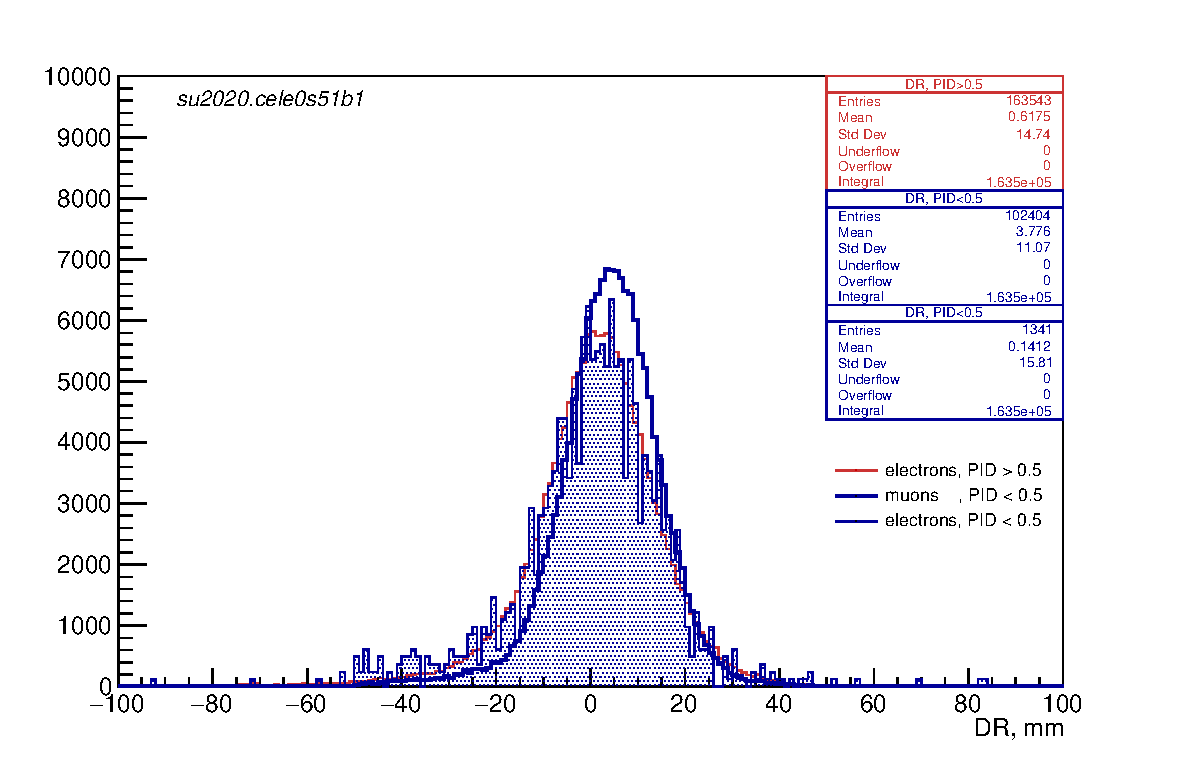
\includegraphics[width=0.60\textwidth]{figures/pdf/figure_00310_pid_emuana_trk_110_vs_111_tch_dr}
      % }
    };
    \node[anchor=south west,inner sep=0] at (10.3,0.) {
      % \node[shift={(0 cm,0.cm)},inner sep=0,rotate={90}] at (0,0) {}
      % \makebox[\textwidth][c] {
      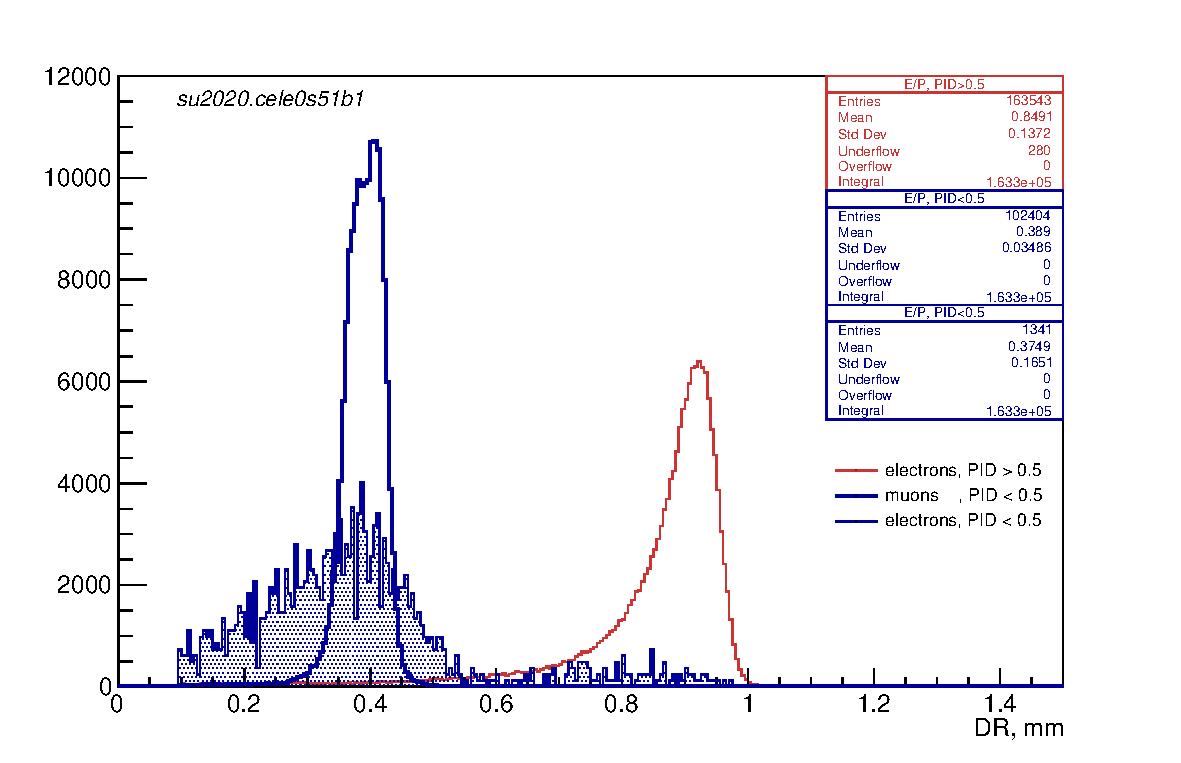
\includegraphics[width=0.60\textwidth]{figures/pdf/figure_00311_pid_emuana_trk_110_vs_111_ep}
      % }
    };
    \node[anchor=south west,inner sep=0] at (0,-7.0) {
      % \node[shift={(0 cm,0.cm)},inner sep=0,rotate={90}] at (0,0) {}
      % \makebox[\textwidth][c] {
      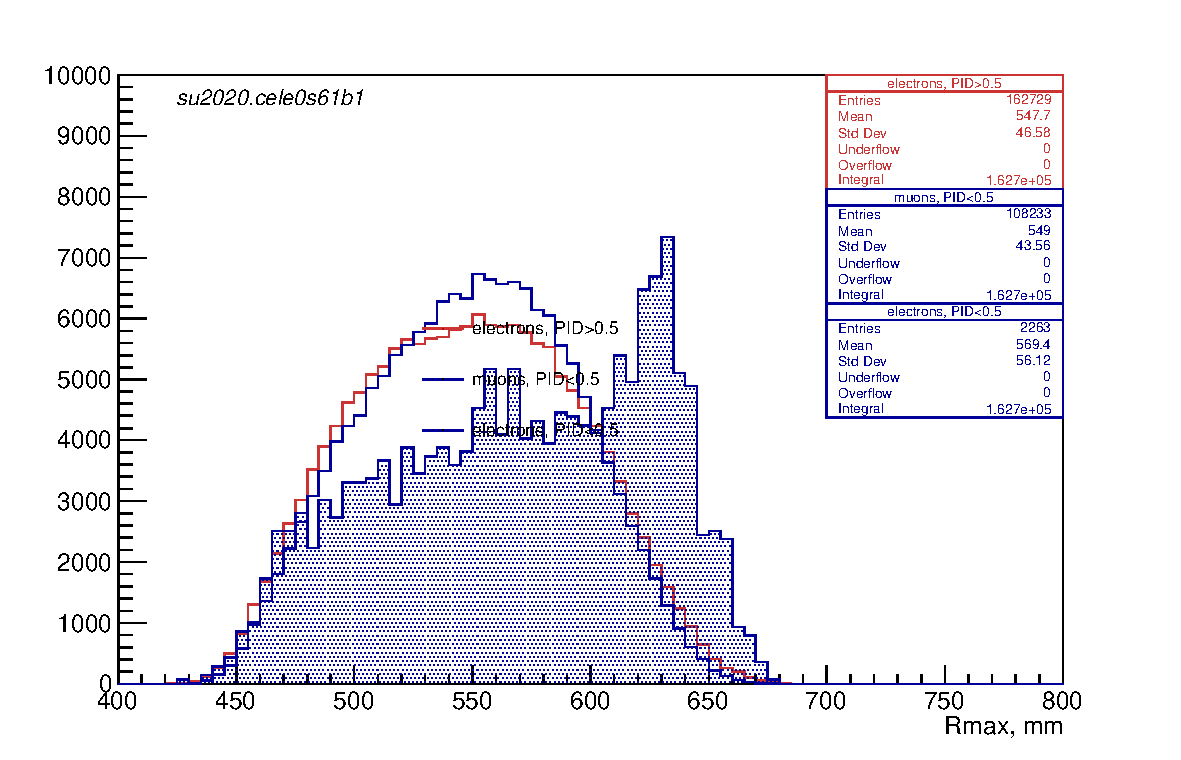
\includegraphics[width=0.60\textwidth]{figures/pdf/figure_00312_pid_emuana_trk_110_vs_111_rmax}
      % }
    };
    \node[anchor=south west,inner sep=0] at (10.3,-7.0) {
      % \node[shift={(0 cm,0.cm)},inner sep=0,rotate={90}] at (0,0) {}
      % \makebox[\textwidth][c] {
      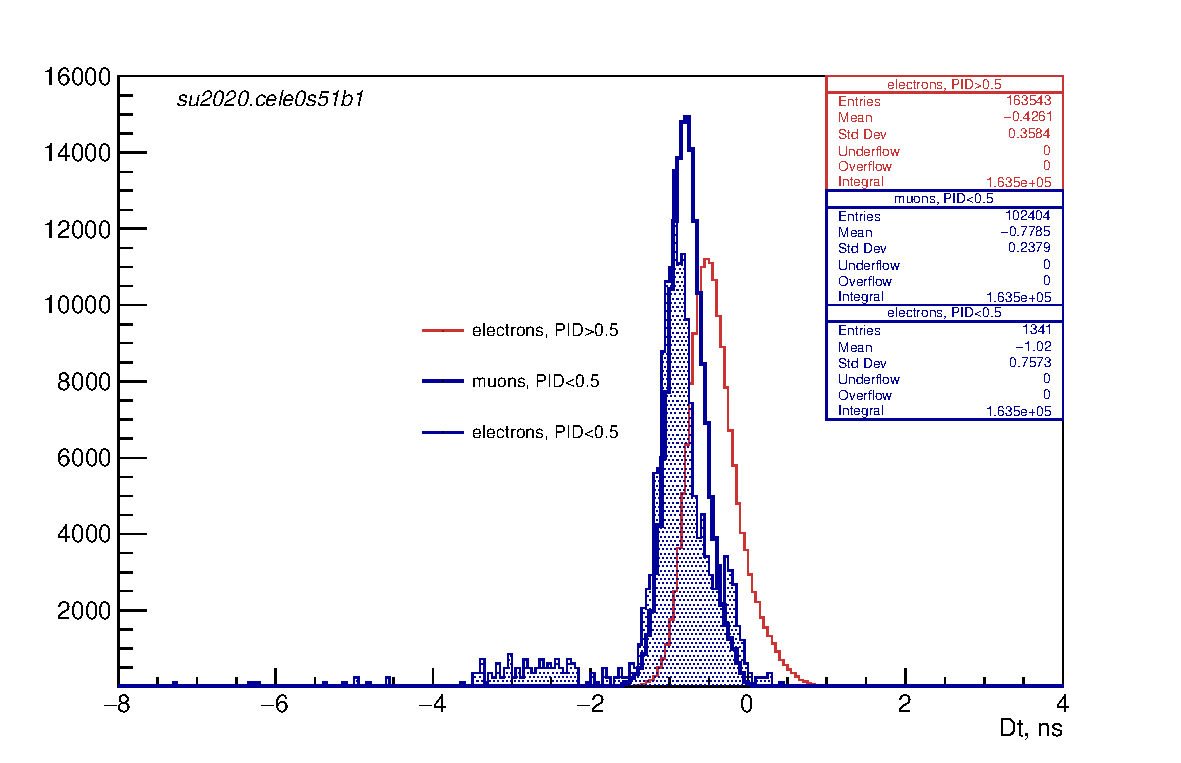
\includegraphics[width=0.60\textwidth]{figures/pdf/figure_00313_pid_emuana_trk_110_vs_111_tch_dt}
      % }
    };
    % \node [text width=6cm, scale=0.8] at (4.5,6.4) {mu2e-18894 by Kevin Lynch and Jim Popp};
  \end{tikzpicture}
  \captionof{figure} {
    \label{fig:electrons_failing_pid}
    % \caption{
    Distributions of the PID variables for electrons passing the PID, muons failing the PID, and electrons failing the PID.
    The PID selection used is $S_{PID} > 0.5$, where $S_{PID}$ is the value of the PID ANN score variable
  }
\end{figure}


%%%%%%%%%%%%%%%%%%%%%%%%%%%%%%%%%%%%%%%%%%%%%%%%%%%%%%%%%%%%%%%%%%%%%%%%%%%%%%
\newpage
\subsection{\MuToEp\ channel}
\label{sec:mumep_channel_pid}
% {\blue lowercase title words after first word}

The PID in \MuToEp\ channel uses a similar ANN trained  using  92 MeV/c positrons and 
positive muons from {\bf pos01s51b0} and {\bf mupl1s51b0} datasets respectively. 
The training procedure is the same as described in Section \ref{sec:mumem_pid_ann_training}.
% 
Figure \ref{fig:pid_score_mumep} shows distributions of the PID ANN score, $S_{PID}$,
for 92 MeV/c positrons and positive muons. About 1.2\% of all muon events have $S_{PID} > 0.5$,
more than 50\% of those events are positrons produced in muon decays in flight.

Plotting the data in log scale - see Figure \ref{fig:pid_score_mumep}(b) - reveals a spike around 0.25,
present in both positron and muon distributions.

% {\red Although the relative contribution of the spike is small, its origin needs to be investigated.}

\begin{figure}[H]
\hspace{-0.6in}
  \begin{tikzpicture}
    \node[anchor=south west,inner sep=0] at (0,0.) {
      % \node[shift={(0 cm,0.cm)},inner sep=0,rotate={90}] at (0,0) {}
      % \makebox[\textwidth][c] {
      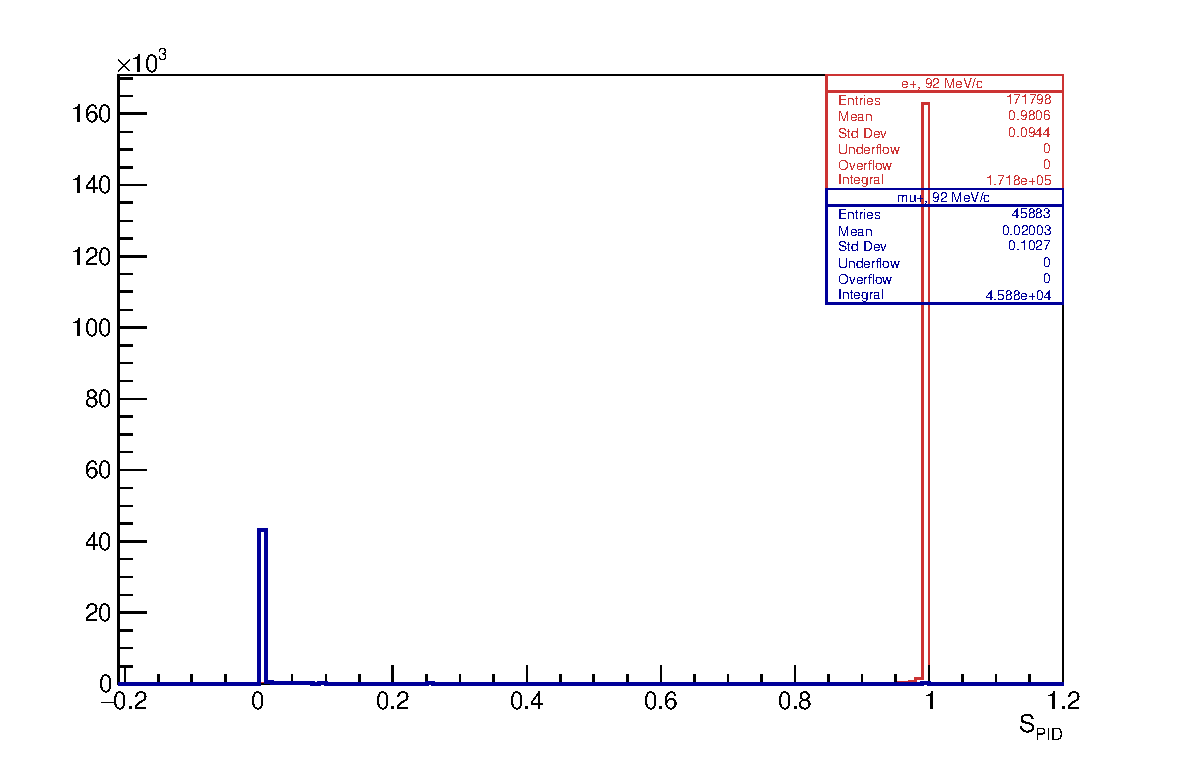
\includegraphics[width=0.60\textwidth]{figures/pdf/figure_00331_su2020_track_ana_1110_trk_219_pidmvaout}
      % }
    };
    \node [text width=1cm, scale=1.0] at (3.,4.5) {(a)};
    \node[anchor=south west,inner sep=0] at (10.5,0.) {
      % \node[shift={(0 cm,0.cm)},inner sep=0,rotate={90}] at (0,0) {}
      % \makebox[\textwidth][c] {
      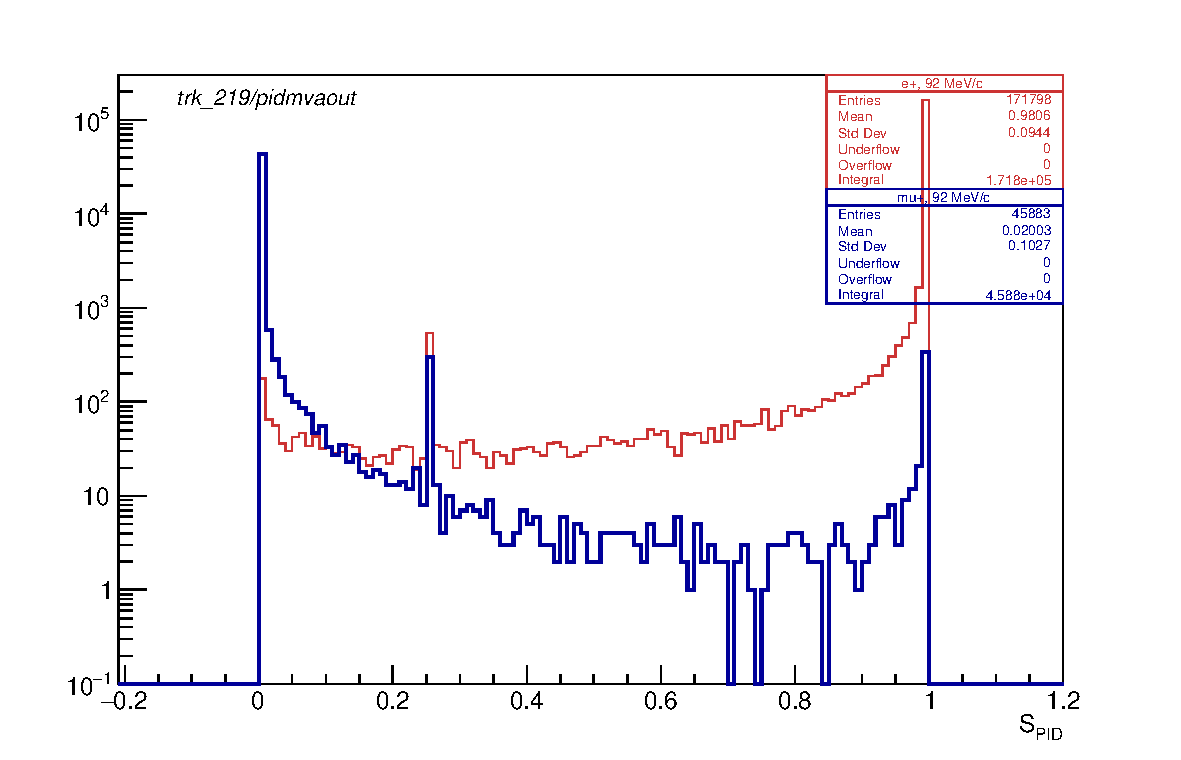
\includegraphics[width=0.60\textwidth]{figures/pdf/figure_00332_su2020_track_ana_1110_trk_219_pidmvaout_log}
      % }
    };
    \node [text width=1cm, scale=1.0] at (13.5,4.5) {(b)};
  \end{tikzpicture}
  \captionof{figure} {
    \label{fig:pid_score_mumep}
    The results of the PID ANN training for the \MuToEp\ channel: the distribution of the PID ANN score, $S_{PID}$,
    for single 92.3 MeV/c positrons and positive muons; (a): linear scale; (b): log scale. \\
    {\red Nature of the spike around 0.25 needs to be investigated.}
  }
\end{figure}

% -*- mode:latex; mode:flyspell -*-


\section{Future work} 
\label{sec:to_be_investigated}

\begin{itemize}
\item 
  investigate the timing systematics in the track-to-cluster matching
\item 
  events with |TCH\_DR|< 100 and no associated clusters, E/P < 0? - a bug in the extrapolation ?
\item
  section \ref{sec:mumep_channel_pid} : spike in the PID score distributions
\item
  section \ref{sec:electrons_failing_pid} : electrons with large value of $R_{max}$
\item
  section \ref{sec:electrons_failing_pid} : electrons with $\Delta{T} < 1.5$ ns
\item
  investigate pros and contras of training the PID ANN in a wider momentum range using
  cosmic datasets
\end{itemize}


\bibliographystyle{unsrtnat}
\bibliography{mu2e_internal_notes,clfv,dio,radiative_muon_capture}
%% \printbibliography
\end{document}


% ------------------------------------------------------------------------------
% templates
% ------------------------------------------------------------------------------
% Table ~\ref{table:summary} gives summary the numbers used in this study.
% 
% \hspace{-0.1in}
% \begin{table}[htbp]
%   \label{table:summary}
%   \begin{center} 
%     {\renewcommand{\arraystretch}{1.0}   % change 1.0 to 1.1 to increase the spacing between the table lines
%       \begin{tabular}{|c|c|c|c|}
%         \hline
%                             & default TS geometry & misaligned TS geometry   &  Ratio(default/misaligned)    \\ 
%         \hline
%         $N_{POT}$            &  $4.96 \cdot 10^6$  &    $5.00 \cdot 10^6$      &   0.992   \\ 
%         $N_{\mu}^{TS3u}$      &  65648              &     61354                 &   1.070   \\ 
%         $N_{\mu}^{TS5}$       &  28517              &     27351                 &   1.043   \\ 
%         $N_{\mu}^{ST}$        &  8868               &      8396                 &   1.056   \\ 
%         $N_{\mu}^{ST}/N_{POT}$ &  $1.79 \pm 0.02$    &    $1.68 \pm 0.02$        &   $1.065 \pm 0.03$        \\ 
%         \hline
%       \end{tabular}
%     }
%   \end{center}
%   \caption{
%     Muons rates at different points of the Mu2e beamline and stopping muon rates for nominal and 
%     misaligned TS geometries
%   }
%   % \vspace{0.5in}
% \end{table}
